\section{Results}

% ____________________________________________________________________________
\subsection{Total cross section and \texorpdfstring{$\BRgamgam/\BRZZ$}{BRgg/BRZZ}}
\label{sec:ratioOfBrsTotalXS}

% hgg:  63.9682042688 +- 9.59143702402
% hzz:  58.2260927627 +- 9.84281414263
% comb: 61.1477521912 +- 7.059056068

The total cross section for Higgs production is measured to be
$61.1   \pm 6.0 \,\text{(stat.)}   \pm 3.7 \,\text{(syst.)}  $\pb
, based on a combination of the total cross sections from $\hgg$ ($64.0\pm9.6$\pb)
and $\hzz$ ($58.2\pm9.8$\pb).
% 
The likelihood scans for the individual decay channels and their combination is shown in
Fig.~\ref{fig:RatioOfbrsAndTotalXSscan}~(\cmsLeft).
% 
The combination result agrees with the current SM value of $55.6\pm2.5$\pb~\cite{deFlorian:2016spz}.

A measurement of the branching fraction of one decay channel is degenerate with a measurement of the total cross section.
% 
However, the ratio of branching fractions for two decay channels can be measured while profiling the total cross section.
% 
The ratio of the $\hgg$ and $\hzz$ branching fractions $R$ is measured to be
$0.092   \pm 0.018 \,\text{(stat.)}   \pm 0.010 \,\text{(syst.)}  $, based on a combination of $\hgg$ and $\hzz$.
% 
This is in agreement with the SM prediction of $0.086$~\cite{deFlorian:2016spz}.
% 
The likelihood scan for $R$ is shown in Fig.~\ref{fig:RatioOfbrsAndTotalXSscan}~(\cmsRight).

\begin{figure}[hbtp]
  \begin{center}
    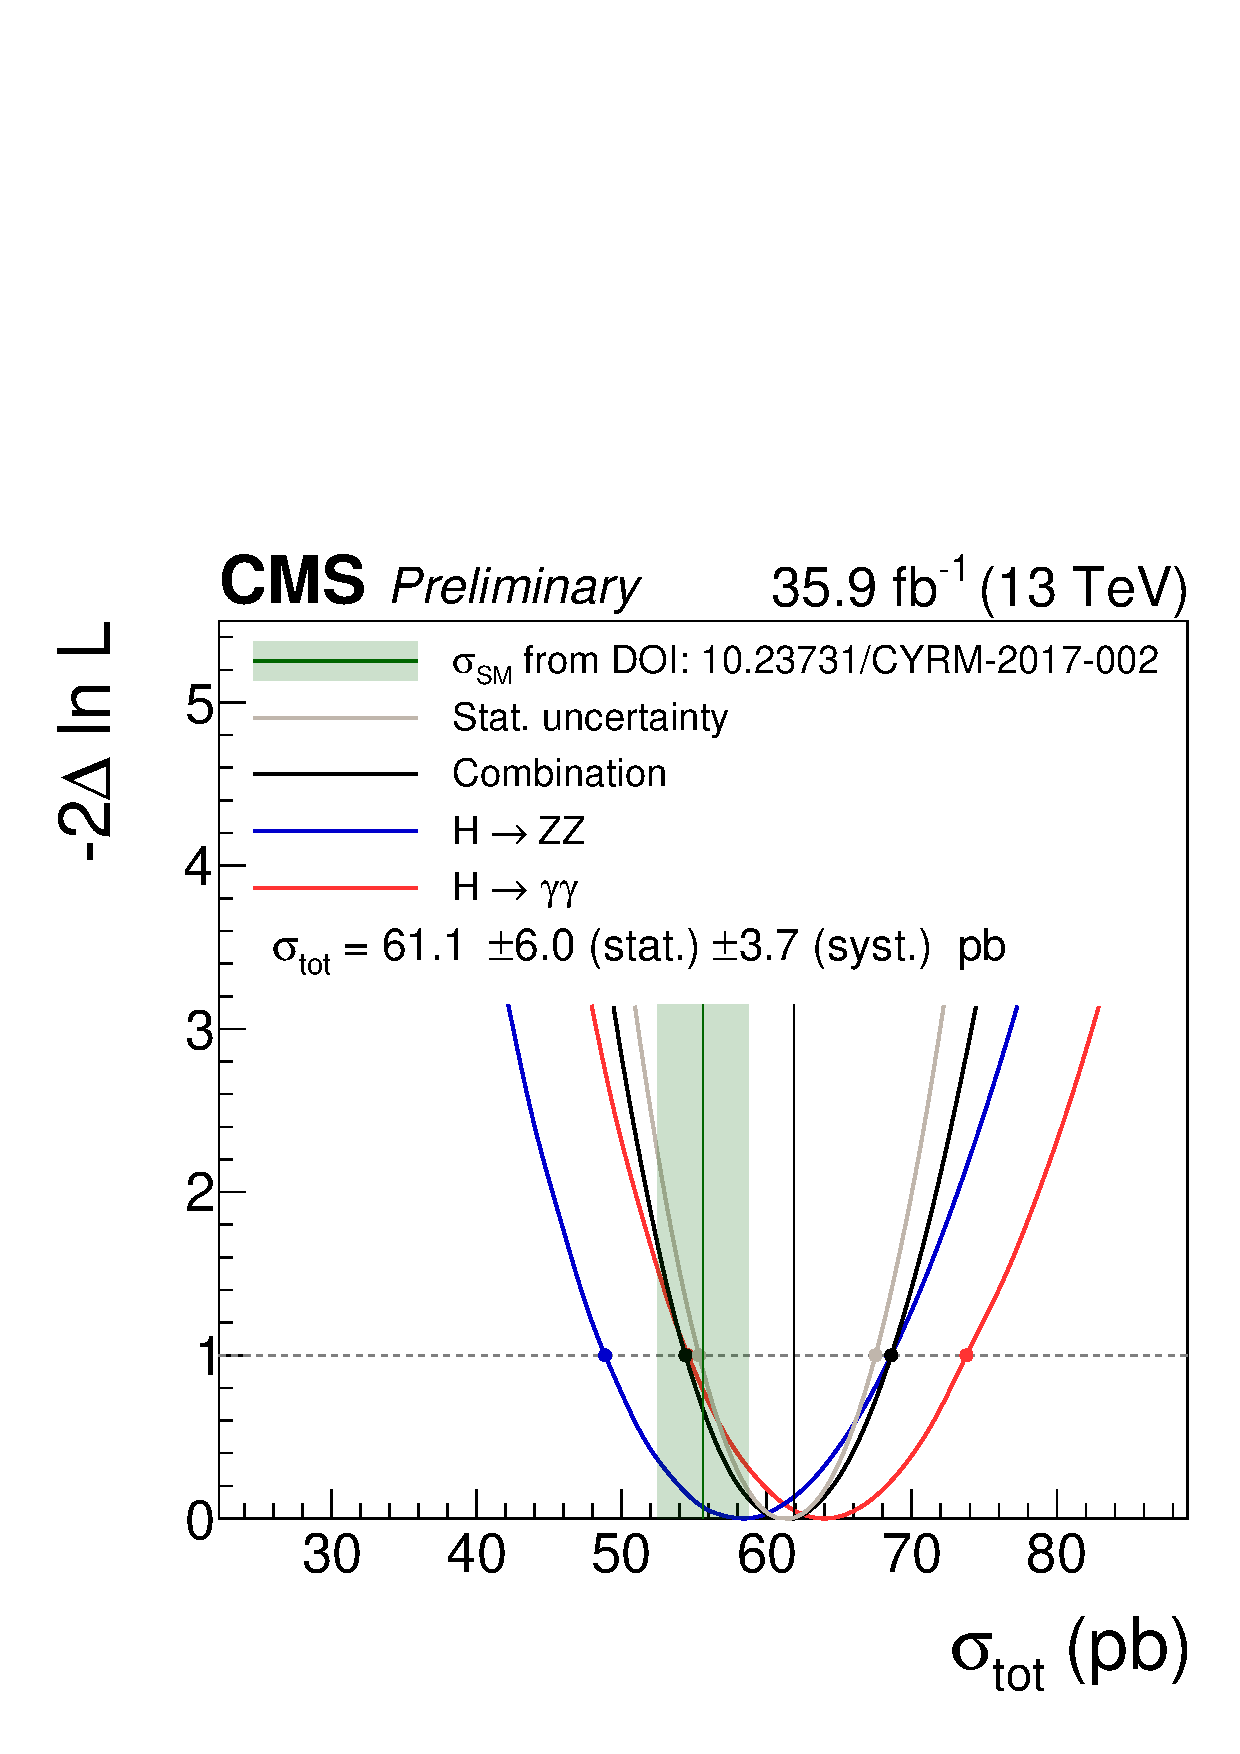
\includegraphics[width=\cmsFigWidth]{img/resultsapproval/reworked/scans_totalXS.pdf}
    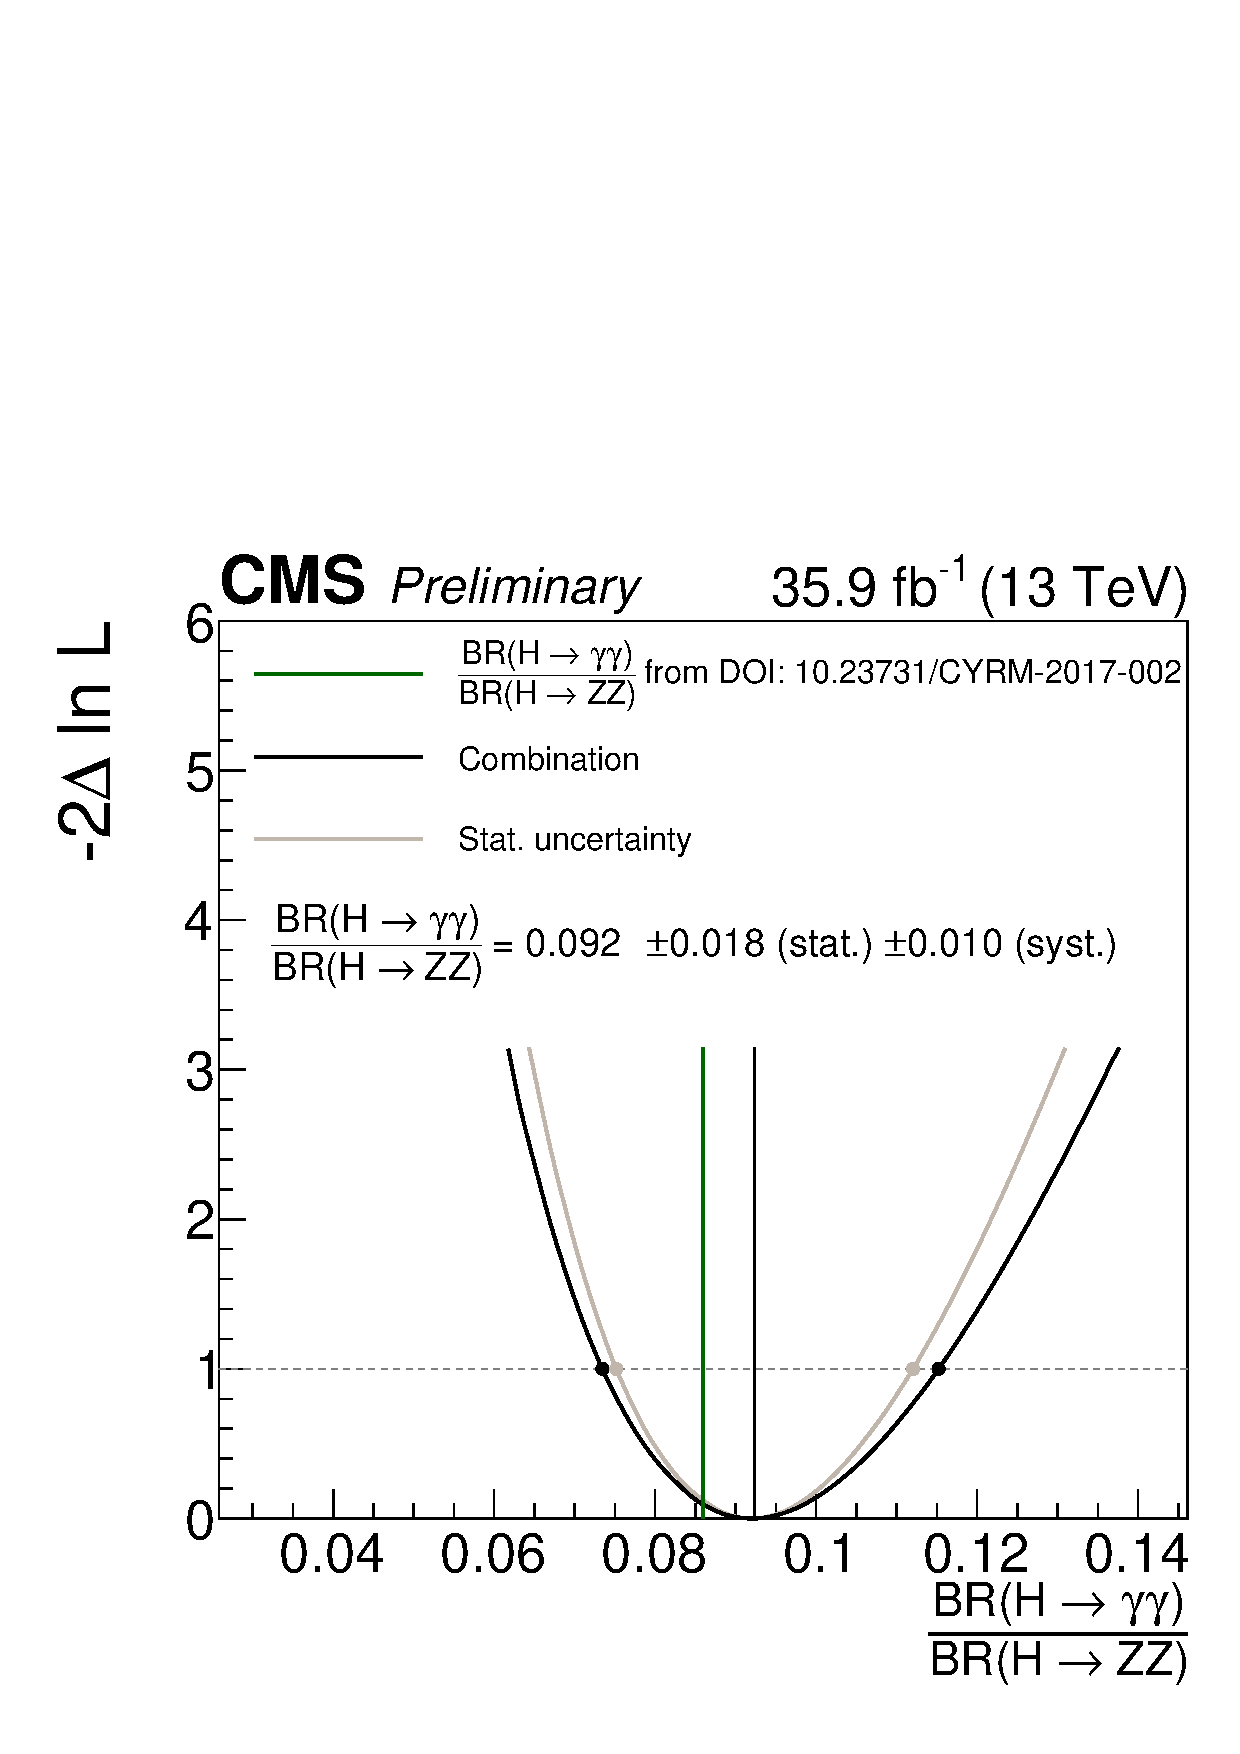
\includegraphics[width=\cmsFigWidth]{img/resultsapproval/reworked/scans_ratioOfBRs.pdf}
    \caption{
        (\cmsLeft) Scan of the total cross section $\sigma_\text{tot}$, based on a combination of the total cross sections from $\hgg$ ($64.0\pm9.6$\pb) and $\hzz$ ($58.2\pm9.8$\pb.
        % 
        (\cmsRight) Scan of the ratio of branching fractions $R$ based on a combination of $\hgg$ and $\hzz$, while profiling all other parameters.
        % 
        The filled markers indicate the one standard deviation interval.
        % 
        % \pasq{
        %     Remove `Preliminary', move legend to the right, move `CMS' to inside the plot. 
        %     }
        % \tk{Will do this later as someone is bound to have comments on this plot anyway.}
        }
    \label{fig:RatioOfbrsAndTotalXSscan}
  \end{center}
\end{figure}


% ____________________________________________________________________________
\subsection{Combinations of differential observables}
\label{sec:noncouplingresults}

The differential cross sections for the observables $\pth$, $\njets$, $\absy$ and $\ptjet$ are shown in
Fig~\ref{fig:CombinedSpectra_pth}, \ref{fig:CombinedSpectra_njets}, \ref{fig:CombinedSpectra_rapidity}, and \ref{fig:CombinedSpectra_ptjet}, including differential cross sections for Higgs production through gluon fusion for the observable $\pth$.
% 
Corresponding bin-to-bin correlation matrices are given in Appendix~\ref{sec:binToBinCorrelationMatrices}.
% 
For the observables $\pth$, $\njets$ and $\ptjet$, the last bin is an overflow bin; here the cross section is given in \pb, and is divided by the bin width of the second-to-last bin (ensuring that if the integrated cross sections in the last and second-to-last bin are equal, the value in the histogram is the same).
% 
Overall no significant deviations from the SM prediction are observed.
% 
For the $\pth$ spectrum, the uncertainties are strongly statistically dominated; in particular, the systematic uncertainty is about half the statistical uncertainty in the last bin, and much smaller in all other bins.
% 
The uncertainty in the combination per bin varies between 30\% and 40\%.
% 
Relative to the spectrum of $\hgg$ alone, the uncertainty decrease achieved by the combination is most notable in the lower $\pt$ region.
% 
% The overall uncertainties vary between 30\% and 40\%, and decrease with respect to the individual decay channels most notably in the lower $\pt$ region.
% % 
% Overall, the uncertainty of the combination with respect to only $\hgg$ is about 15\% smaller.
% 
The contribution of $\hbb$ to the overall precision of the combination is strongest in the last $\pth$ bin.

\begin{figure}[hbtp]
  \begin{center}
    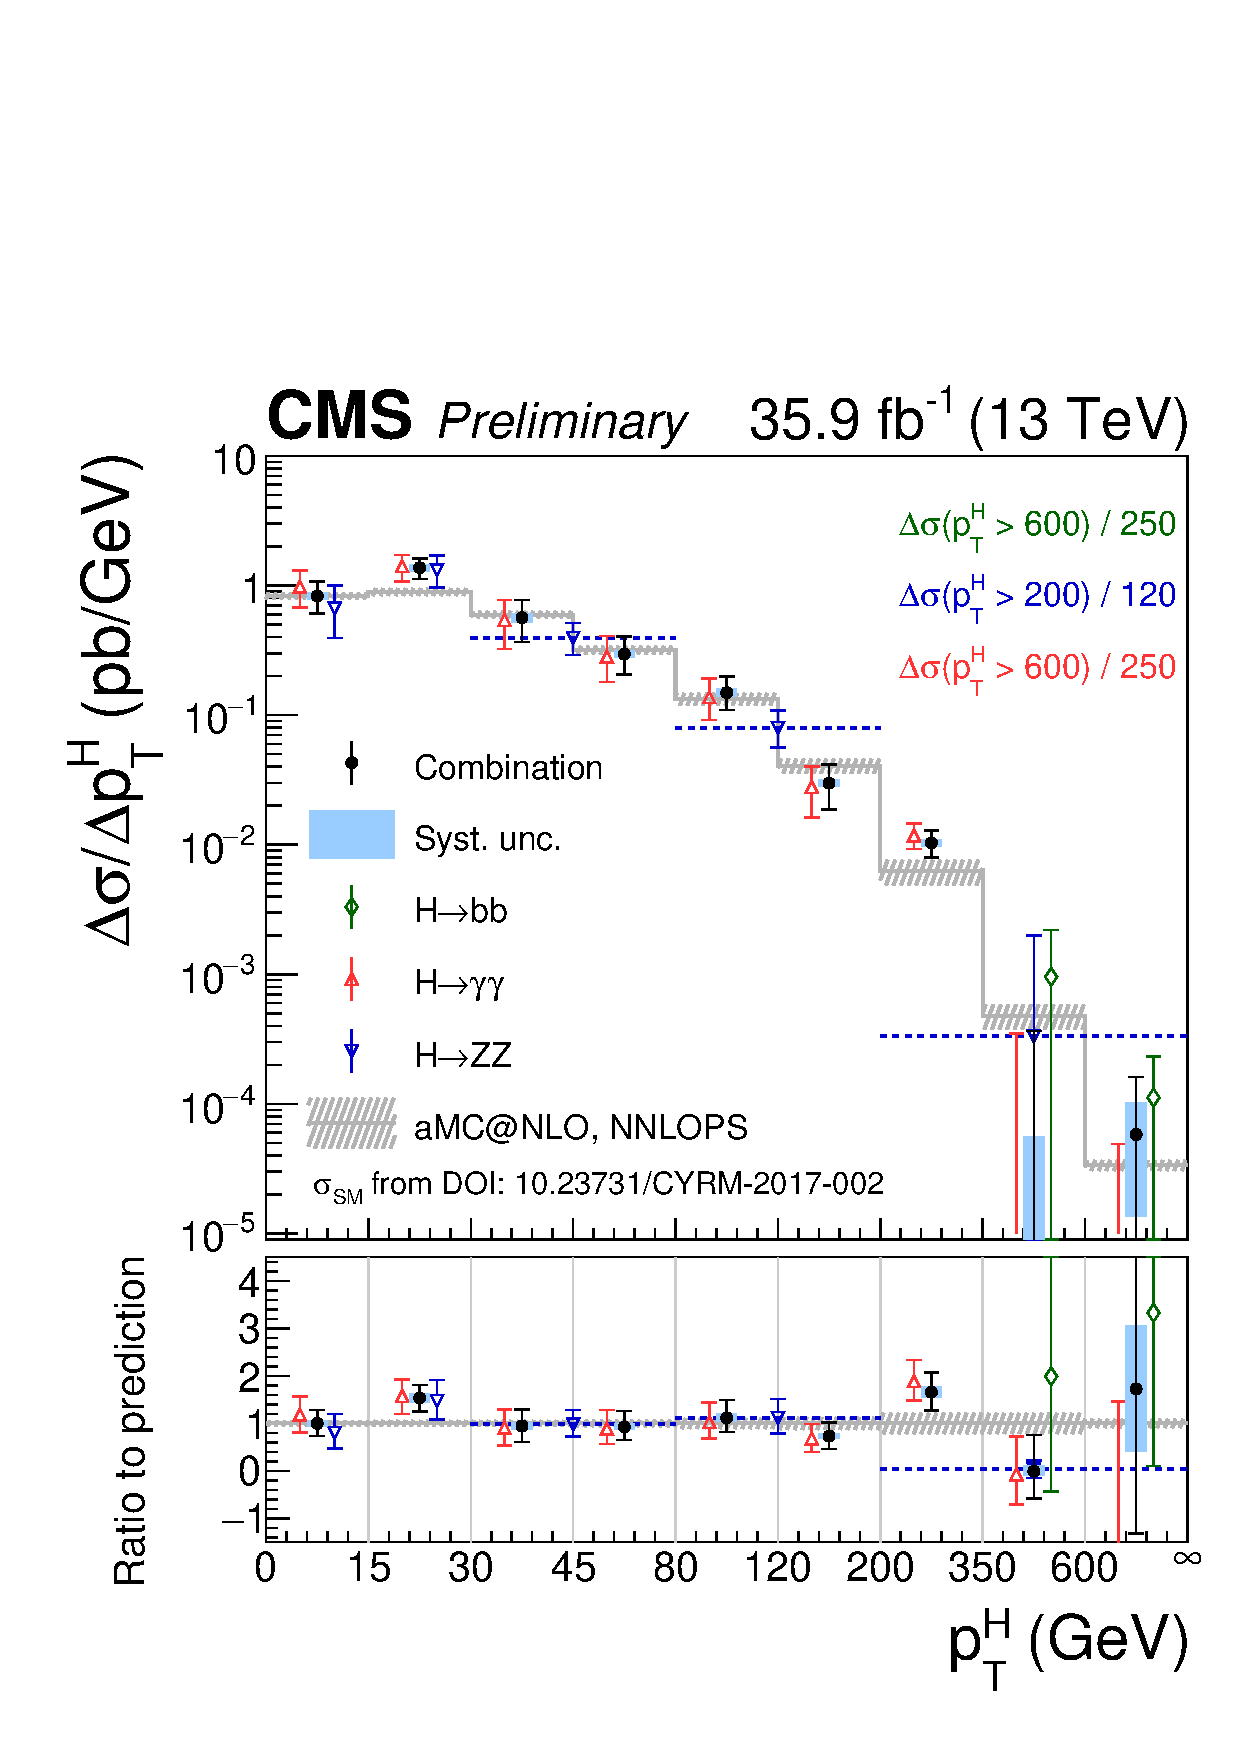
\includegraphics[width=\cmsFigWidth]{img/resultsapproval/reworked/spectra_pth_smH.pdf}
    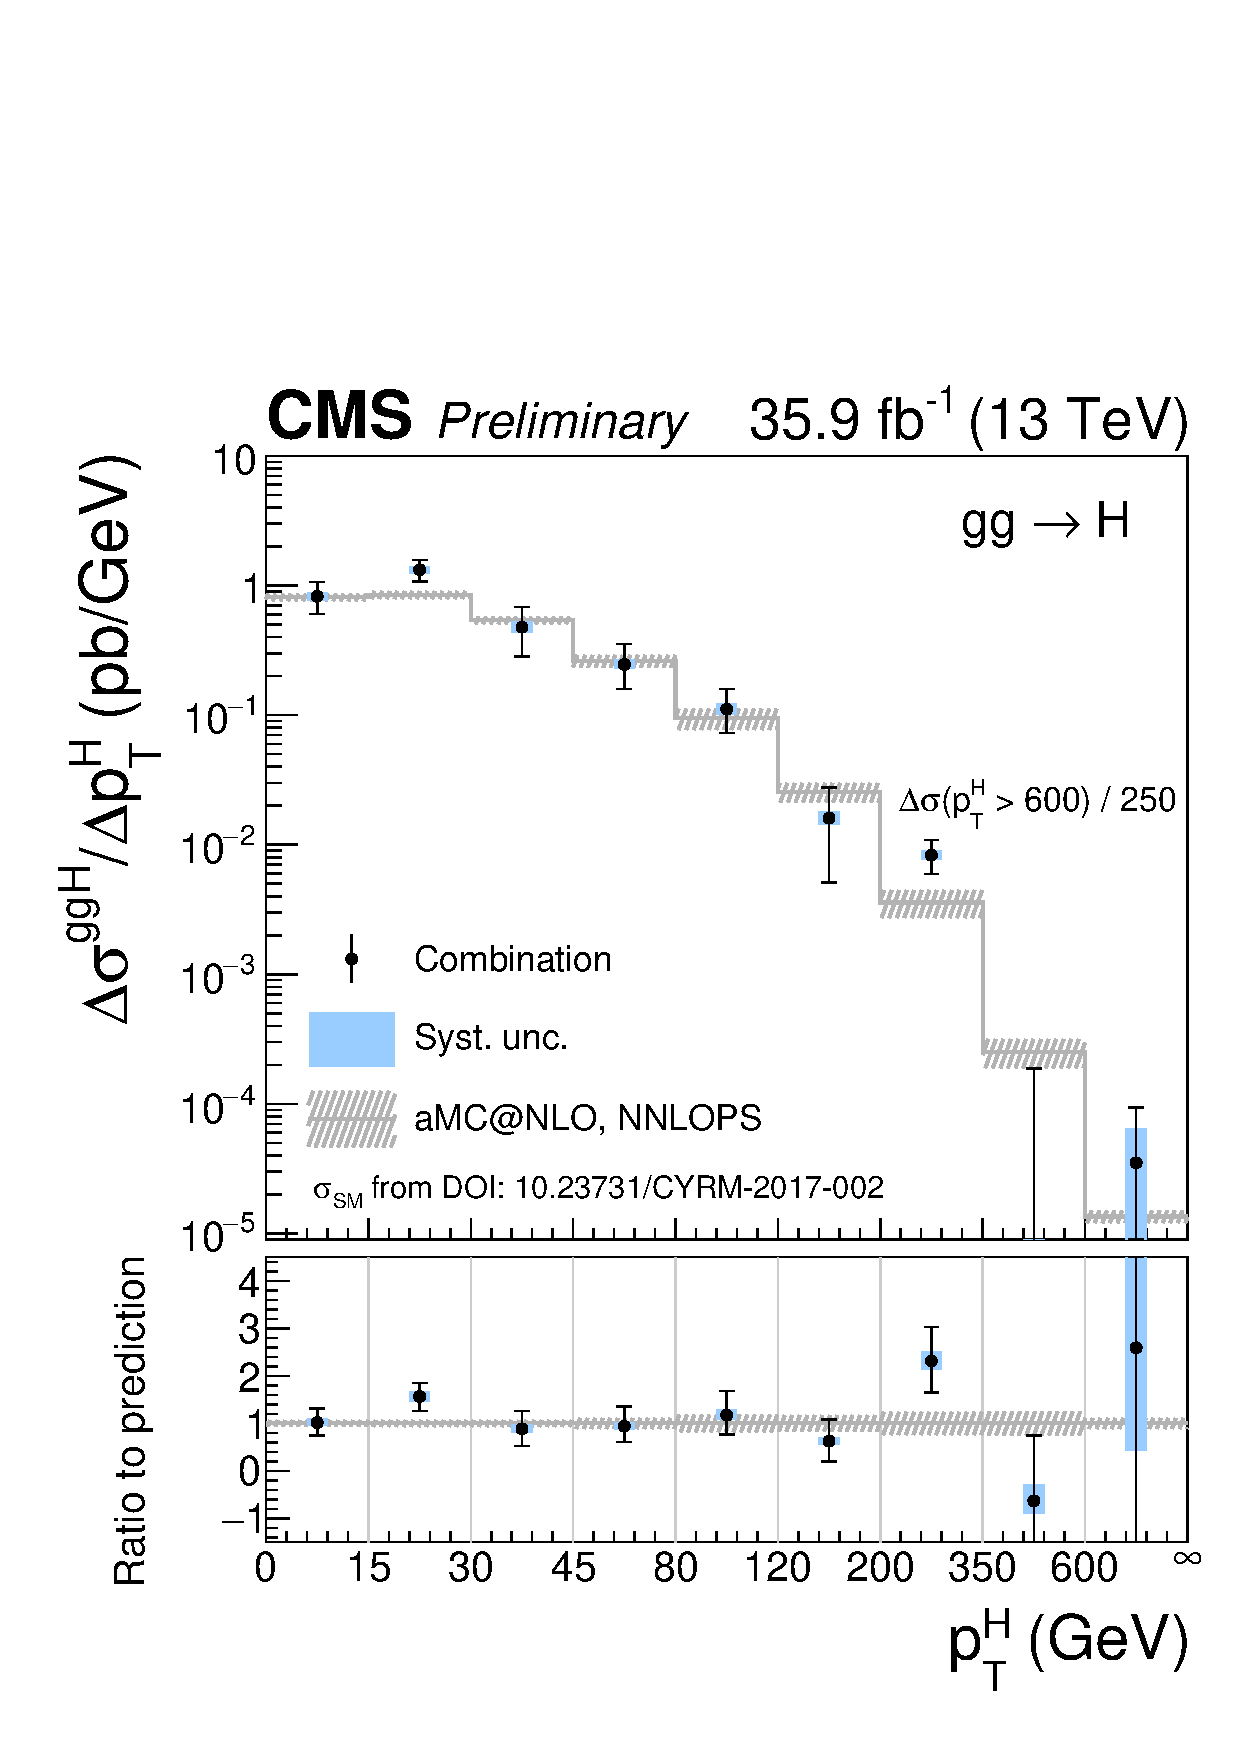
\includegraphics[width=\cmsFigWidth]{img/resultsapproval/reworked/spectra_pth_ggH.pdf}
    \caption{
        Best fit values and uncertainties of the cross sections and signal strengths.
        % 
        (\cmsLeft) $\pth$.
        (\cmsRight) $\pth$ while fixing non-gluon-fusion contributions to their SM expectation.
        % 
        % \pasq{Different markers per spectrum, integrals need to be bigger and different.
        % }
        % \tk{Will do this later as someone is bound to have comments on this plot anyway.}
        }
    \label{fig:CombinedSpectra_pth}
  \end{center}
\end{figure}

\begin{figure}[hbtp]
  \begin{center}
    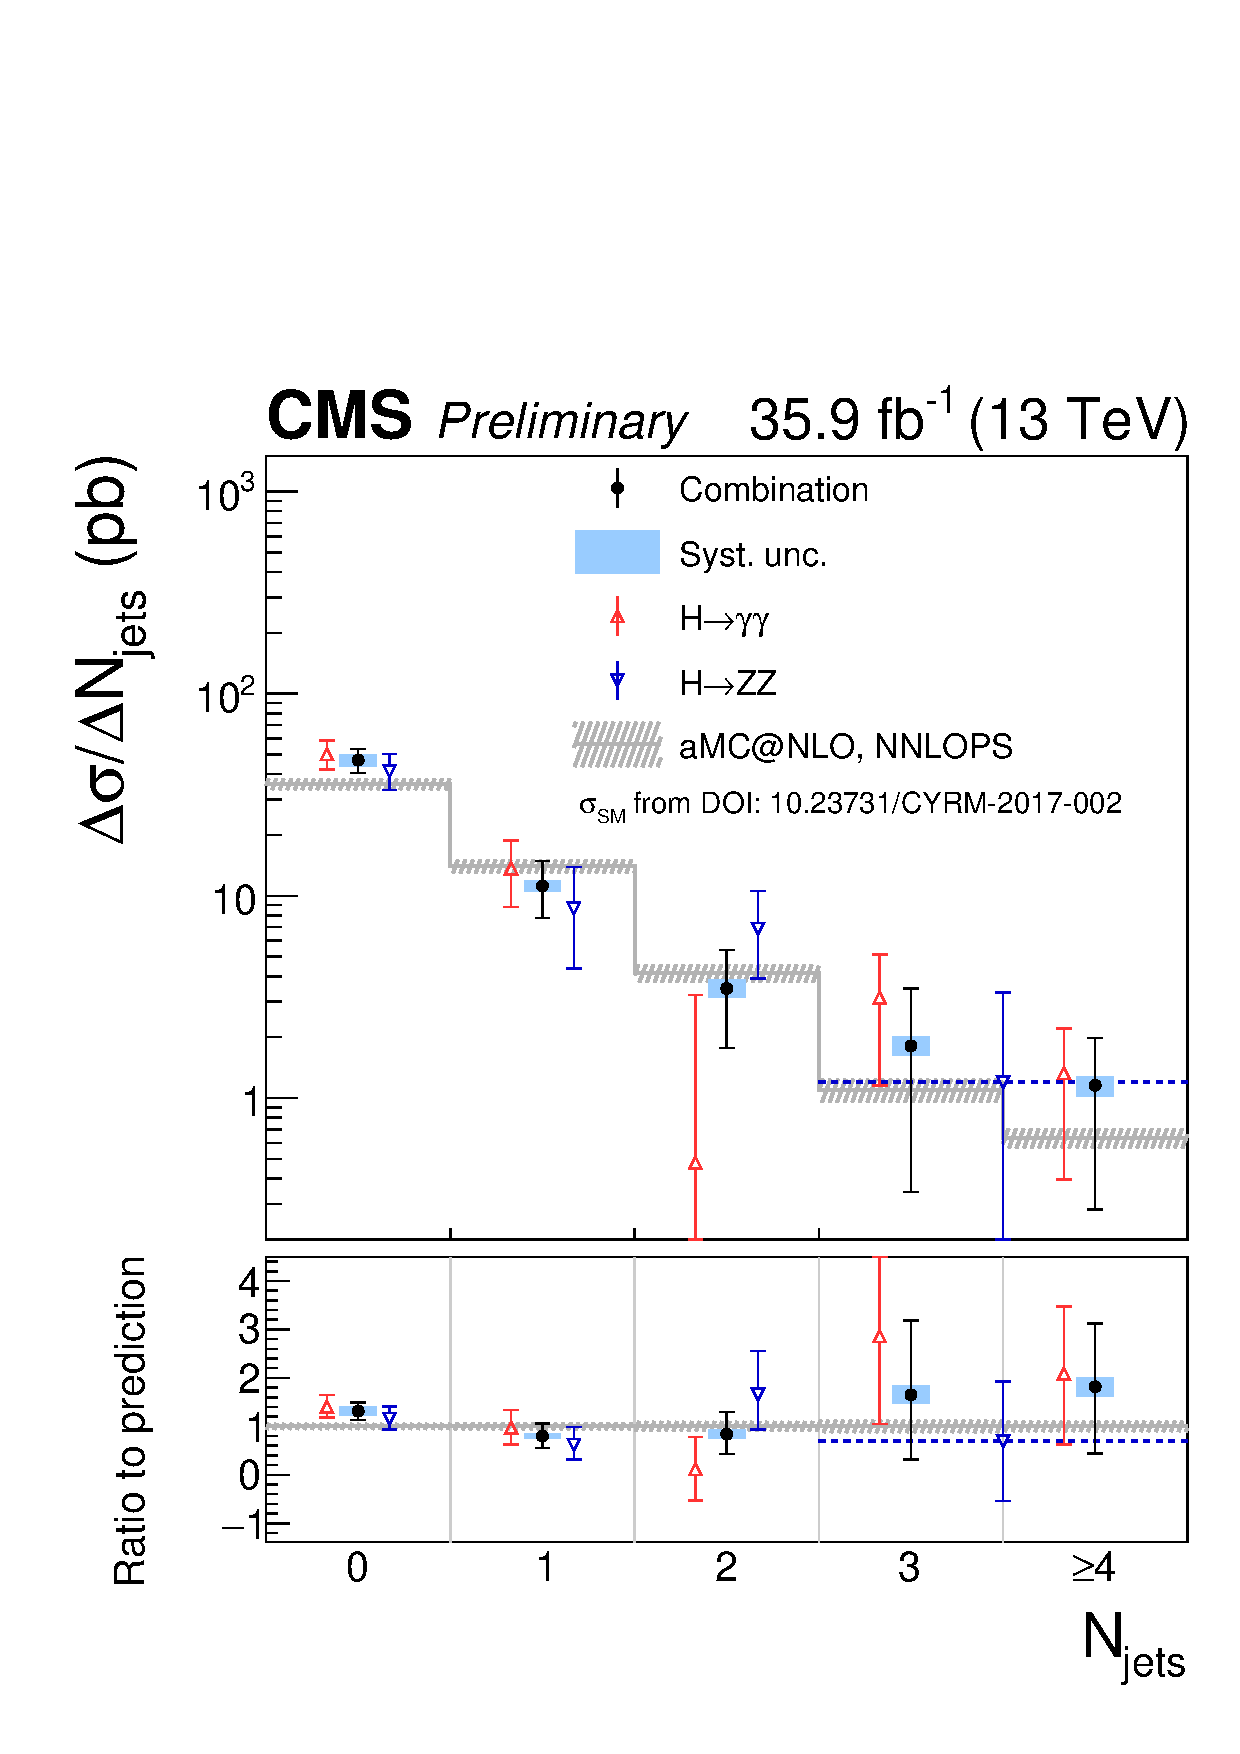
\includegraphics[width=\cmsFigWidth]{img/resultsapproval/reworked/spectra_njets.pdf}
    \caption{
        Best fit values and uncertainties of the cross sections and signal strengths for the $\njets$-spectrum.
        }
    \label{fig:CombinedSpectra_njets}
  \end{center}
\end{figure}

\begin{figure}[hbtp]
  \begin{center}
    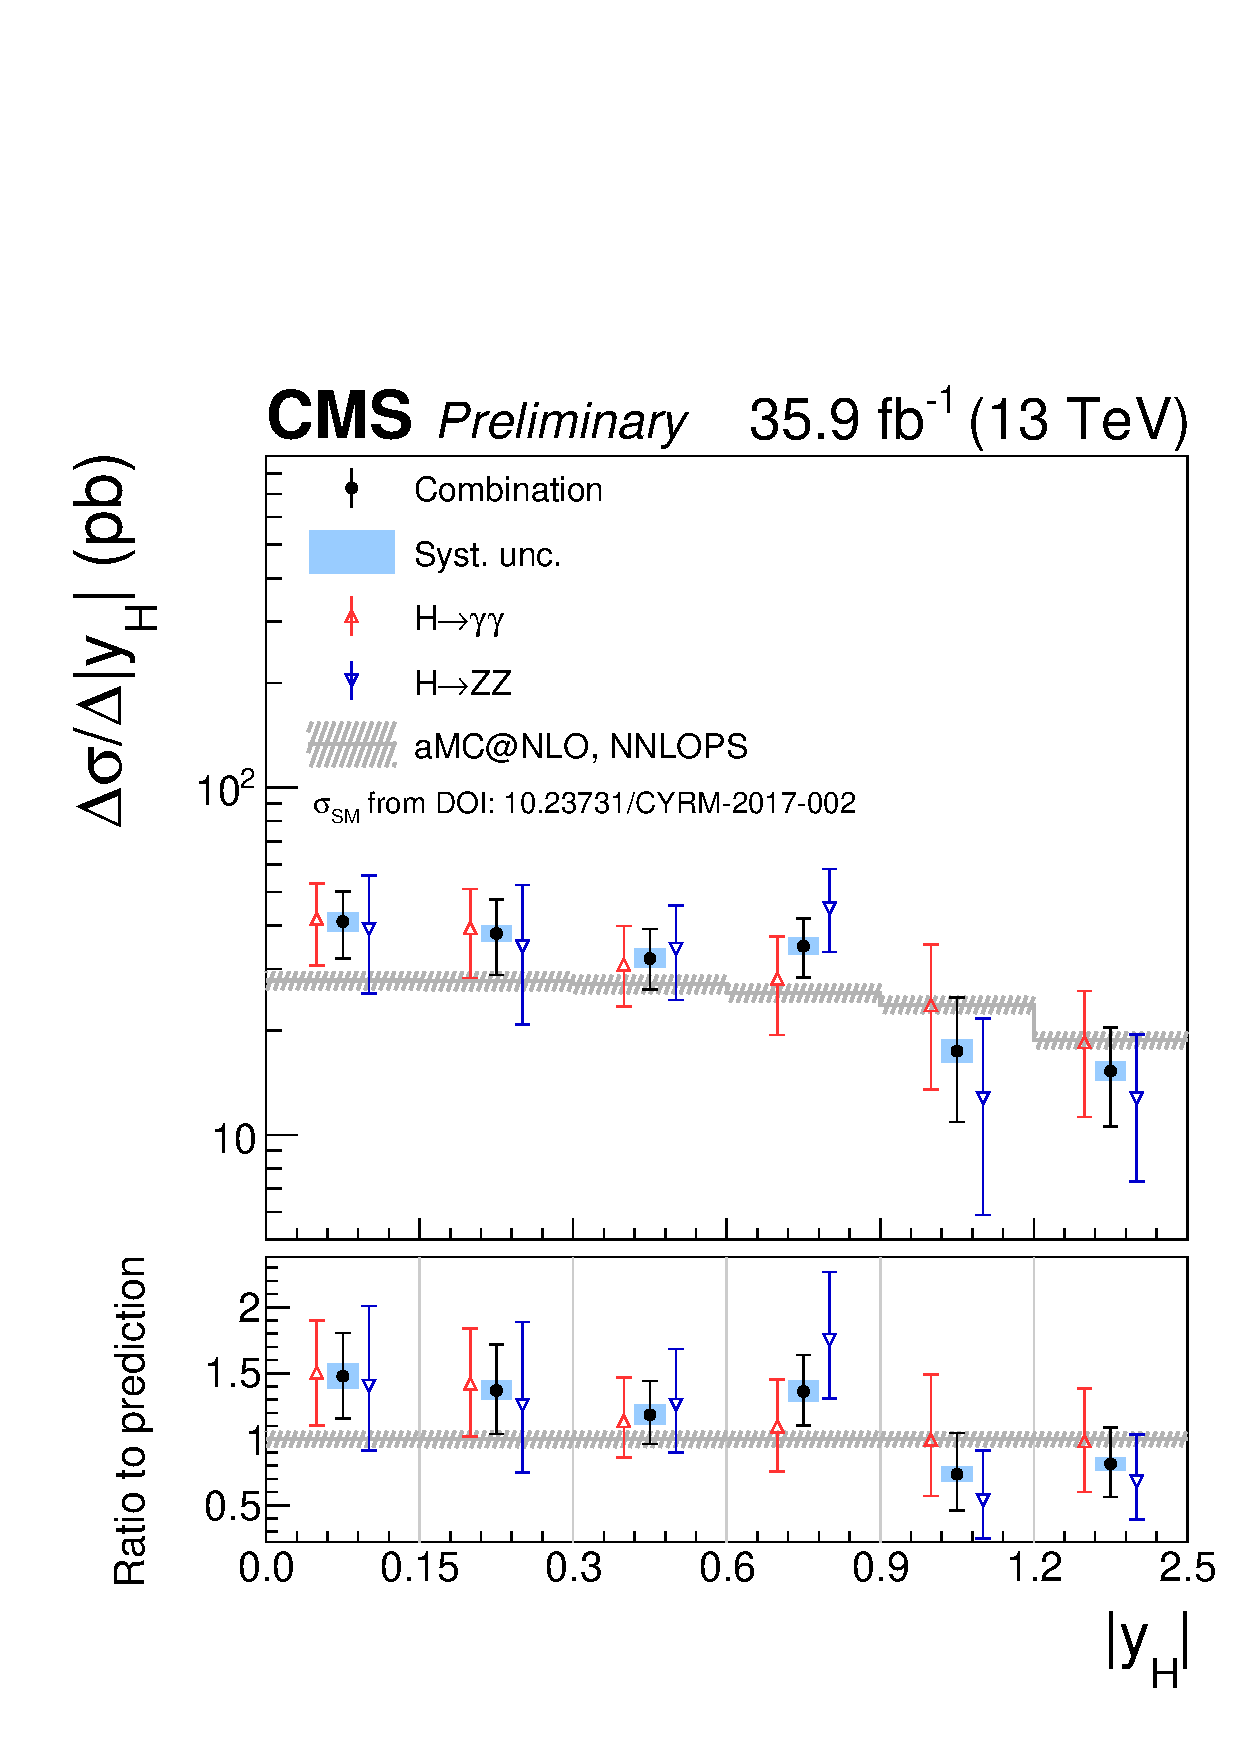
\includegraphics[width=\cmsFigWidth]{img/resultsapproval/reworked/spectra_rapidity.pdf}
    \caption{
        Expected best fit values and uncertainties of the cross sections and signal strengths for the $\absy$-spectrum.
        }
    \label{fig:CombinedSpectra_rapidity}
  \end{center}
\end{figure}

\begin{figure}[hbtp]
  \begin{center}
    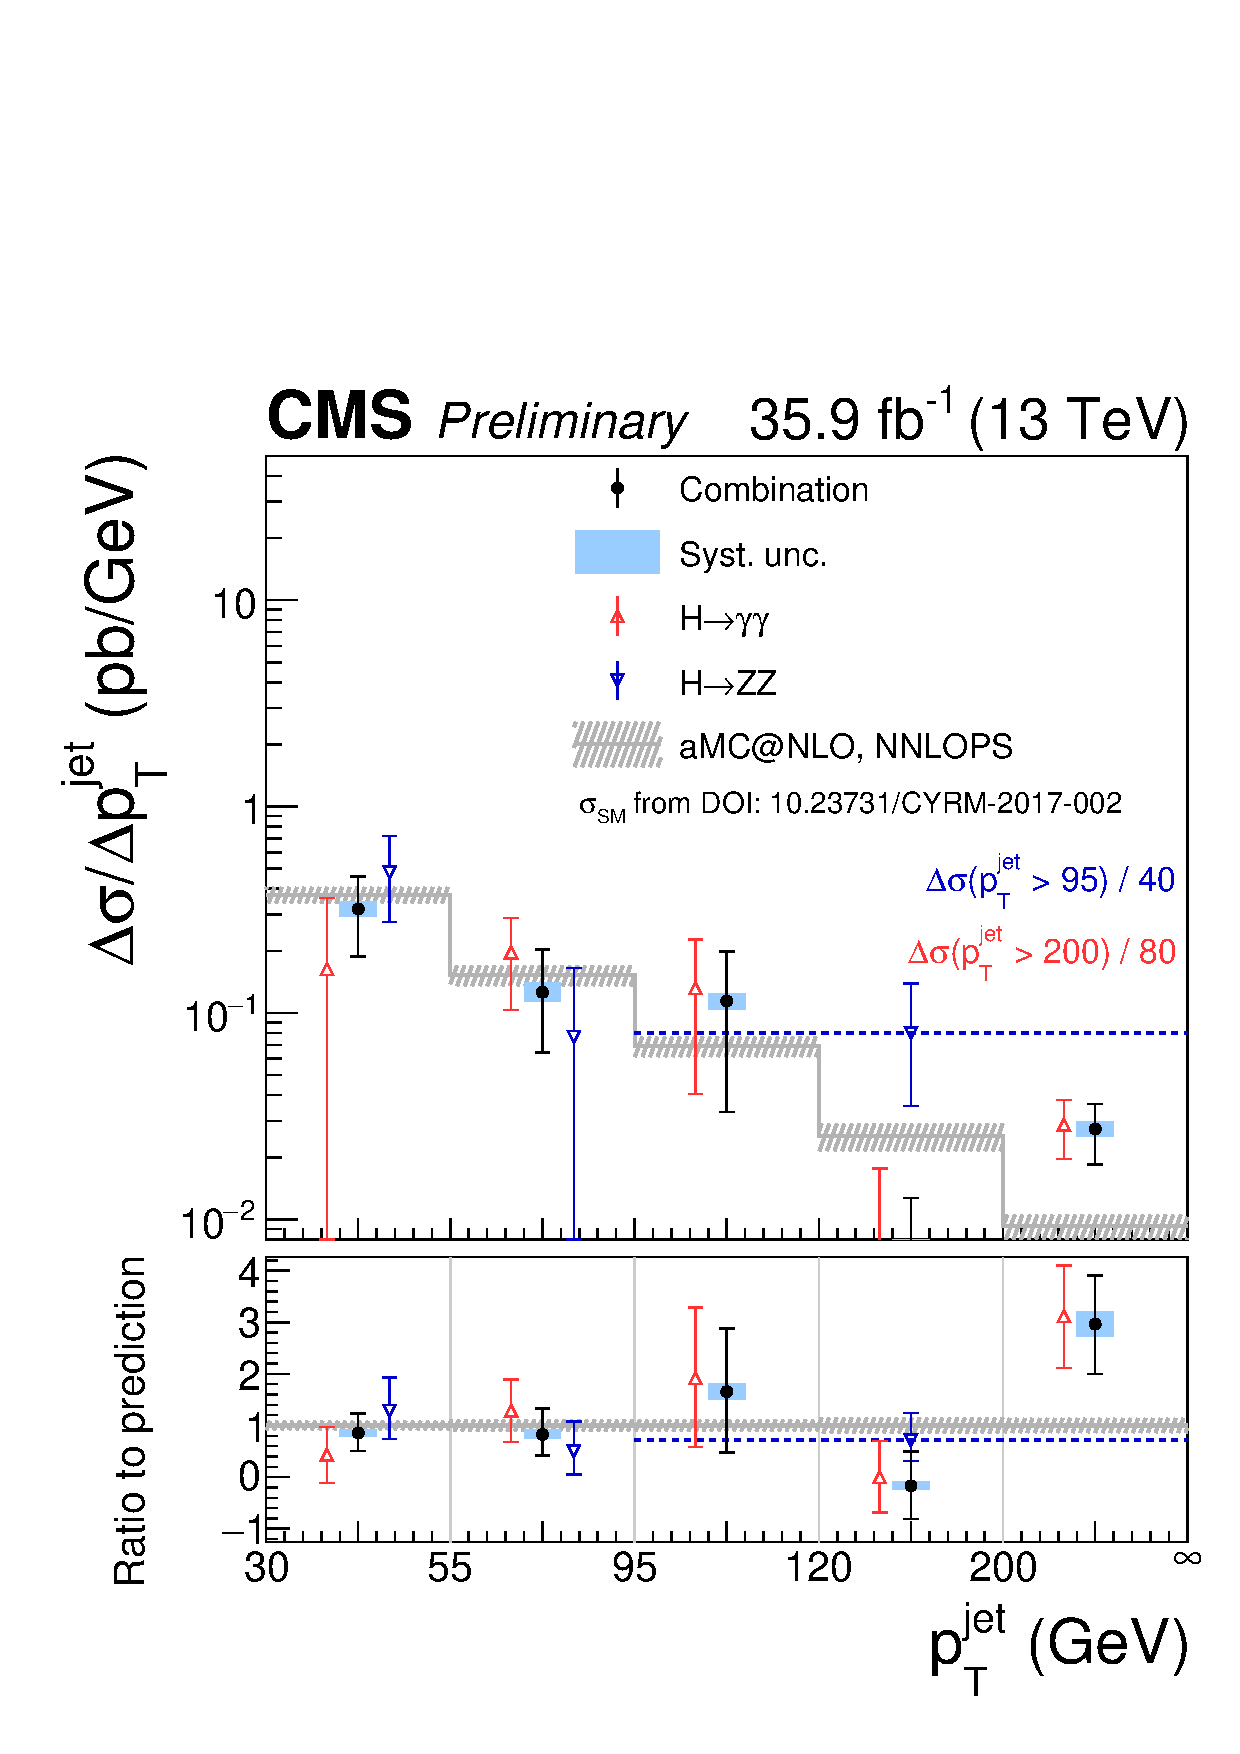
\includegraphics[width=\cmsFigWidth]{img/resultsapproval/reworked/spectra_ptjet.pdf}
    \caption{
        Expected best fit values and uncertainties of the cross sections and signal strengths for the $\ptjet$-spectrum.
        }
    \label{fig:CombinedSpectra_ptjet}
  \end{center}
\end{figure}


% ____________________________________________________________________________
\toggledclearpage
\subsection{Fits of Higgs coupling modifiers: \texorpdfstring{$\kappa_b$}{kb} vs. \texorpdfstring{$\kappa_c$}{kc}}
\label{sec:ResultsKappabKappac}

Figure~\ref{fig:scans_kappabkappac_nominal}(\cmsLeft) shows the one and two standard deviation contours of the fit of the $\kappa_b/\kappa_c$ parametrization from Ref.~\cite{Bishara:2016jga} to data.
% using the likelihood function described in Sec.~\ref{sec:statisticalanalysis}
% , including the contours obtained using only the $\hgg$ or $\hzz$ data.
% 
The calculations from Ref.~\cite{Bishara:2016jga} are given up to the scale of the Higgs mass, and thus $\hbb$ (whose $\pth$ spectrum starts at $\pth=350$\GeV) is not used as input for the results obtained here.
% 
% \arc{``which the parametrization for κb and κc is specified'' $\rightarrow$ you mean in the paper ? In addition you can say why it is not reliable theoretically, if the argument is given somewhere.}
% 
% Hence it is not included the $\kappa_b$ vs. $\kappa_c$ log-likelihood fit.
% 
The bin-to-bin correlations of the theoretical uncertainties are implemented as described in Sec.~\ref{sec:systematics}. 
% 
% 
The substructure on the combined scan shows a ring shape around the origin, and an almost one standard deviation agreement with the SM prediction.
% 
% 
% The substructure on the combined scan shows a ring shape around the origin, in which the origin and the SM expectation are not included, although these points are contained in the region allowed at $2\sigma$.
% 
% A comparable proof-of-concept study was already performed in Ref.~\cite{Bishara:2016jga} using ATLAS data from Run I, yielding the overall bounds $\kappa_c \in [ -16, 18 ]$.~\tk{Edit here posssibly.}

% img/resultsapproval/reworked/multicont_Yukawa_couplingdependentBRs.pdf
% img/resultsapproval/reworked/multicont_Yukawa_floatingBRs.pdf


In order to evaluate the effect of the shape on the constraints on $\kappa_b$ and $\kappa_c$, the procedure is repeated with freely floating branching fractions, effectively removing constraints from the total width and from the overall normalization.
% 
The result of this fit is shown in Fig.~\ref{fig:scans_kappabkappac_nominal}(\cmsLeft).
% 
As expected, the range of allowed values of $\kappa_b$ and $\kappa_c$ is much wider than in the case of coupling-dependent branching fractions.


\begin{figure}[hbtp]
  \begin{center}
    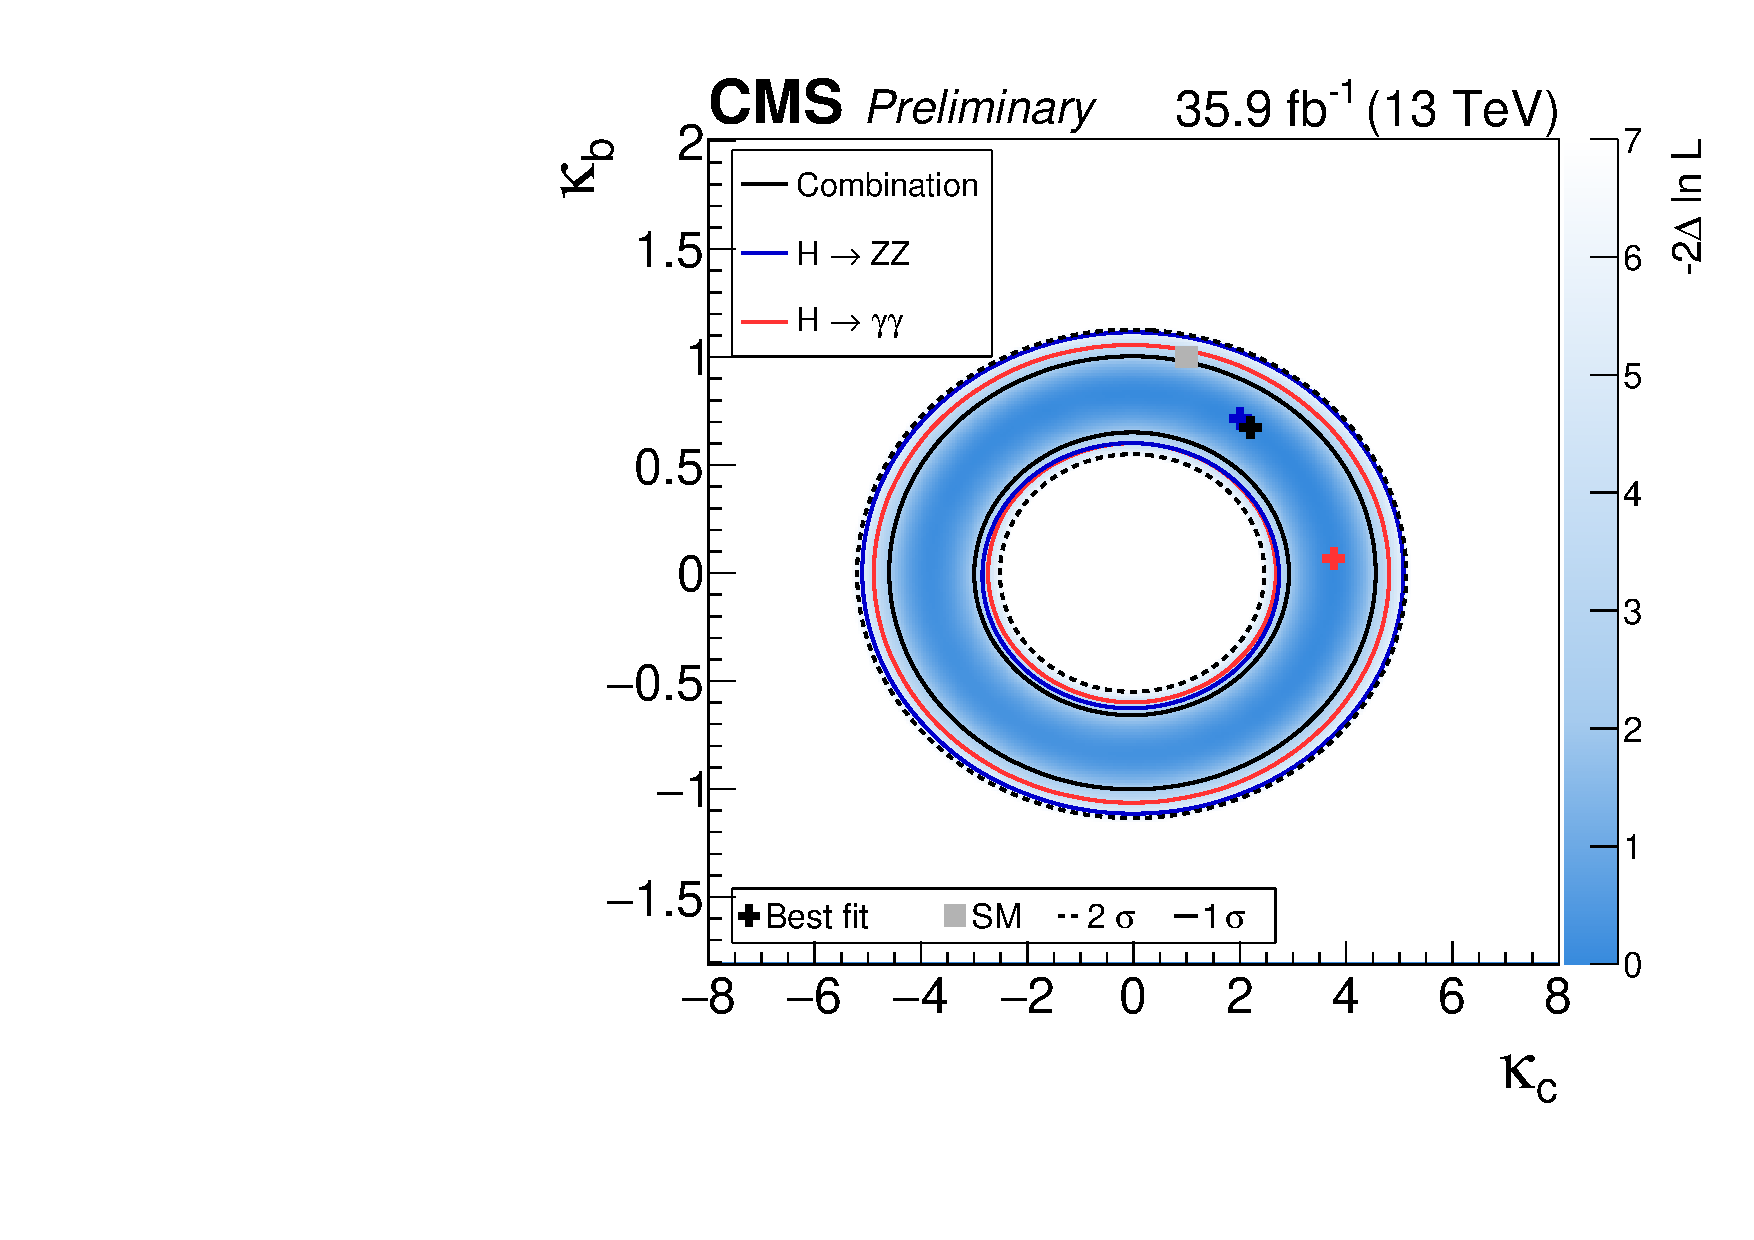
\includegraphics[width=0.49\linewidth]{img/resultsapproval/reworked/multicont_Yukawa_couplingdependentBRs.pdf}
    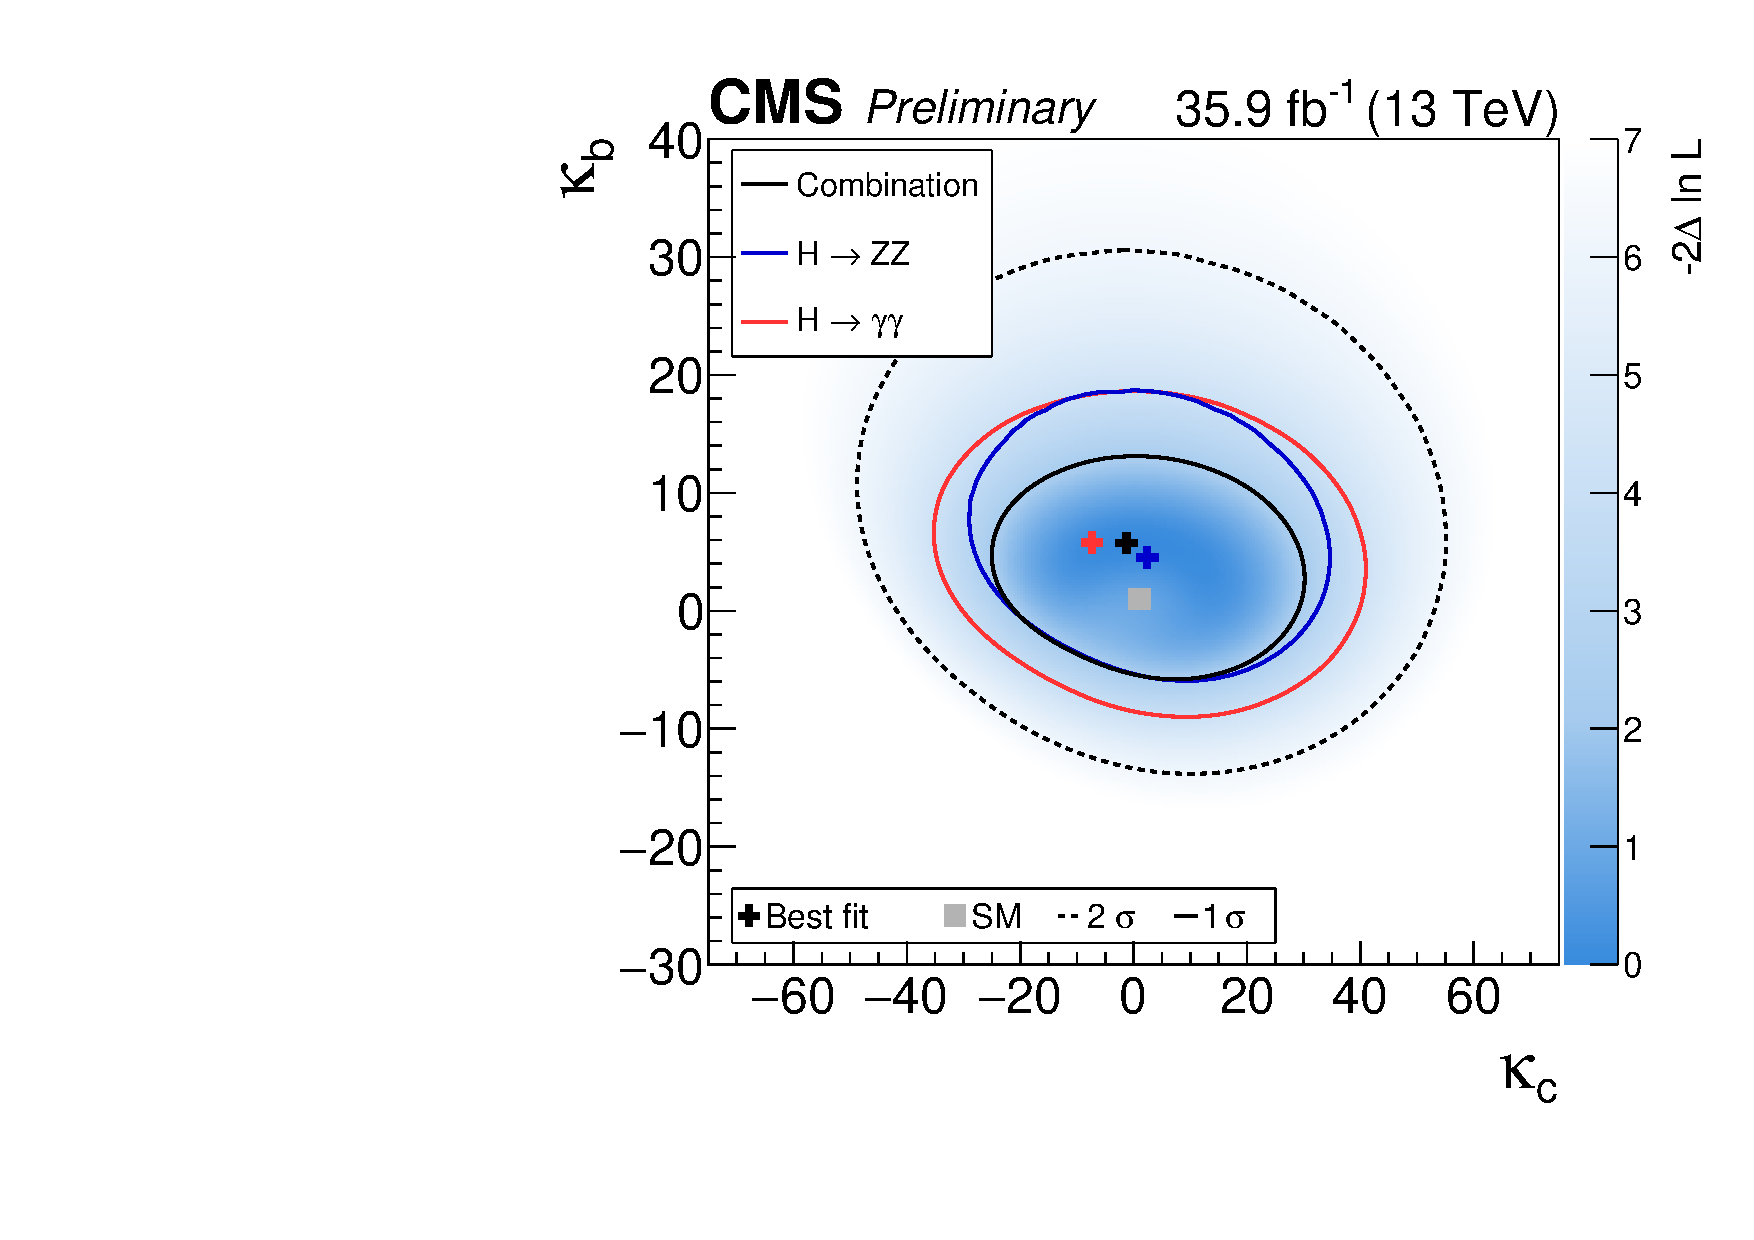
\includegraphics[width=0.49\linewidth]{img/resultsapproval/reworked/multicont_Yukawa_floatingBRs.pdf}
    % 
    \caption{
        Simultaneous fit results for $\kappa_b$ and $\kappa_c$.
        % 
        (\cmsLeft) One and two standard deviation contours are shown for the combined ($\hgg$ and $\hzz$) fit to data and for $\hgg$ and $\hzz$ separately, assuming a coupling dependency of the branching fractions.
        % 
        (\cmsRight) One and two standard deviation contours are shown for the combined ($\hgg$ and $\hzz$) fit to data and for $\hgg$ and $\hzz$ separately, assuming freely floating branching fractions.
        % 
        % 
        % Simultaneous fit results for $\kappa_b$ and $\kappa_c$, showing one- and two-$\sigma$ contours for the fit to data.
        % % 
        % % including fit results using only the $\hgg$ and $\hzz$ inputs.
        % % 
        % (\cmsLeft) Branching fractions scaling with $\kappa_b$ and $\kappa_c$.
        % % 
        % (\cmsRight) Branching fractions freely floating, effectively yielding the constraint obtained solely from the shape.
        }
    \label{fig:scans_kappabkappac_nominal}
  \end{center}
\end{figure}


Separate limits can be set on $\kappa_b$ and $\kappa_c$ by profiling one coupling and scanning over the other.
% 
% Limits on $\kappa_b$ and $\kappa_c$ individually can be set by profiling one coupling and scanning over the other.
% 
The results of these single-coupling scans are shown in Fig.~\ref{fig:scans_kappabkappac_oneDimScans} and Fig.~\ref{fig:scans_kappabkappac_oneDimScans_scenario2}.
% 
The observed uncertainties in the one-dimensional scans are:
% 
% \clearpage
\begin{equation}
\label{eq:kappasensitivity}
\begin{array}{c}
\kappabLeftObserved < \kappa_b < \kappabRightObserved  \quad(\kappabLeftAsimov < \kappa_b < \kappabRightAsimov \;\; \text{expected})  \,,
\\[8pt]
\kappacLeftObserved < \kappa_c < \kappacRightObserved \quad(\kappacLeftAsimov < \kappa_c < \kappacRightAsimov \;\; \text{expected})
\,,
\end{array}
\end{equation}
% 
in the case of branching fractions that depend on $\kappa_b$ and $\kappa_c$, and
% 
\begin{equation}
\label{eq:kappasensitivity}
\begin{array}{c}
\kappabLeftObservedFLOATINGBRS < \kappa_b < \kappabRightObservedFLOATINGBRS  \quad(\kappabLeftAsimovFLOATINGBRS < \kappa_b < \kappabRightAsimovFLOATINGBRS \;\; \text{expected})  \,,
\\[8pt]
\kappacLeftObservedFLOATINGBRS < \kappa_c < \kappacRightObservedFLOATINGBRS \quad(\kappacLeftAsimovFLOATINGBRS < \kappa_c < \kappacRightAsimovFLOATINGBRS \;\; \text{expected})
\,,
\end{array}
\end{equation}
% 
in the case of freely floated branching fractions.
% 
For the coupling-dependent branching fractions, the results are shaped predominantly by constraints from the total width rather than by distortions of the $\pth$ spectrum.
% 
If the branching fractions are fixed to their SM expectations, the one-dimensional scans yield the following expected uncertainties:
% 
\begin{equation}
\label{eq:kappasensitivity_fixedSMBRs}
\begin{array}{c}
-1.9 < \kappa_b < 2.9 \;\; (\text{expected})  \,,
 \\[8pt]
-8.7 < \kappa_c < 10.6 \;\; (\text{expected})
\,.
\end{array}
\end{equation}
% 
These limits are comparable to those in Ref.~\cite{Bishara:2016jga}, where $\kappa_c \in [ -16, 18 ]$, noting that the results here are based on a larger data set.
% 
The limits obtained are competitive with the limits from other direct search channels summarized in Sec.~\ref{sec:introduction}.


\begin{figure}[Hbtp]
  \begin{center}
    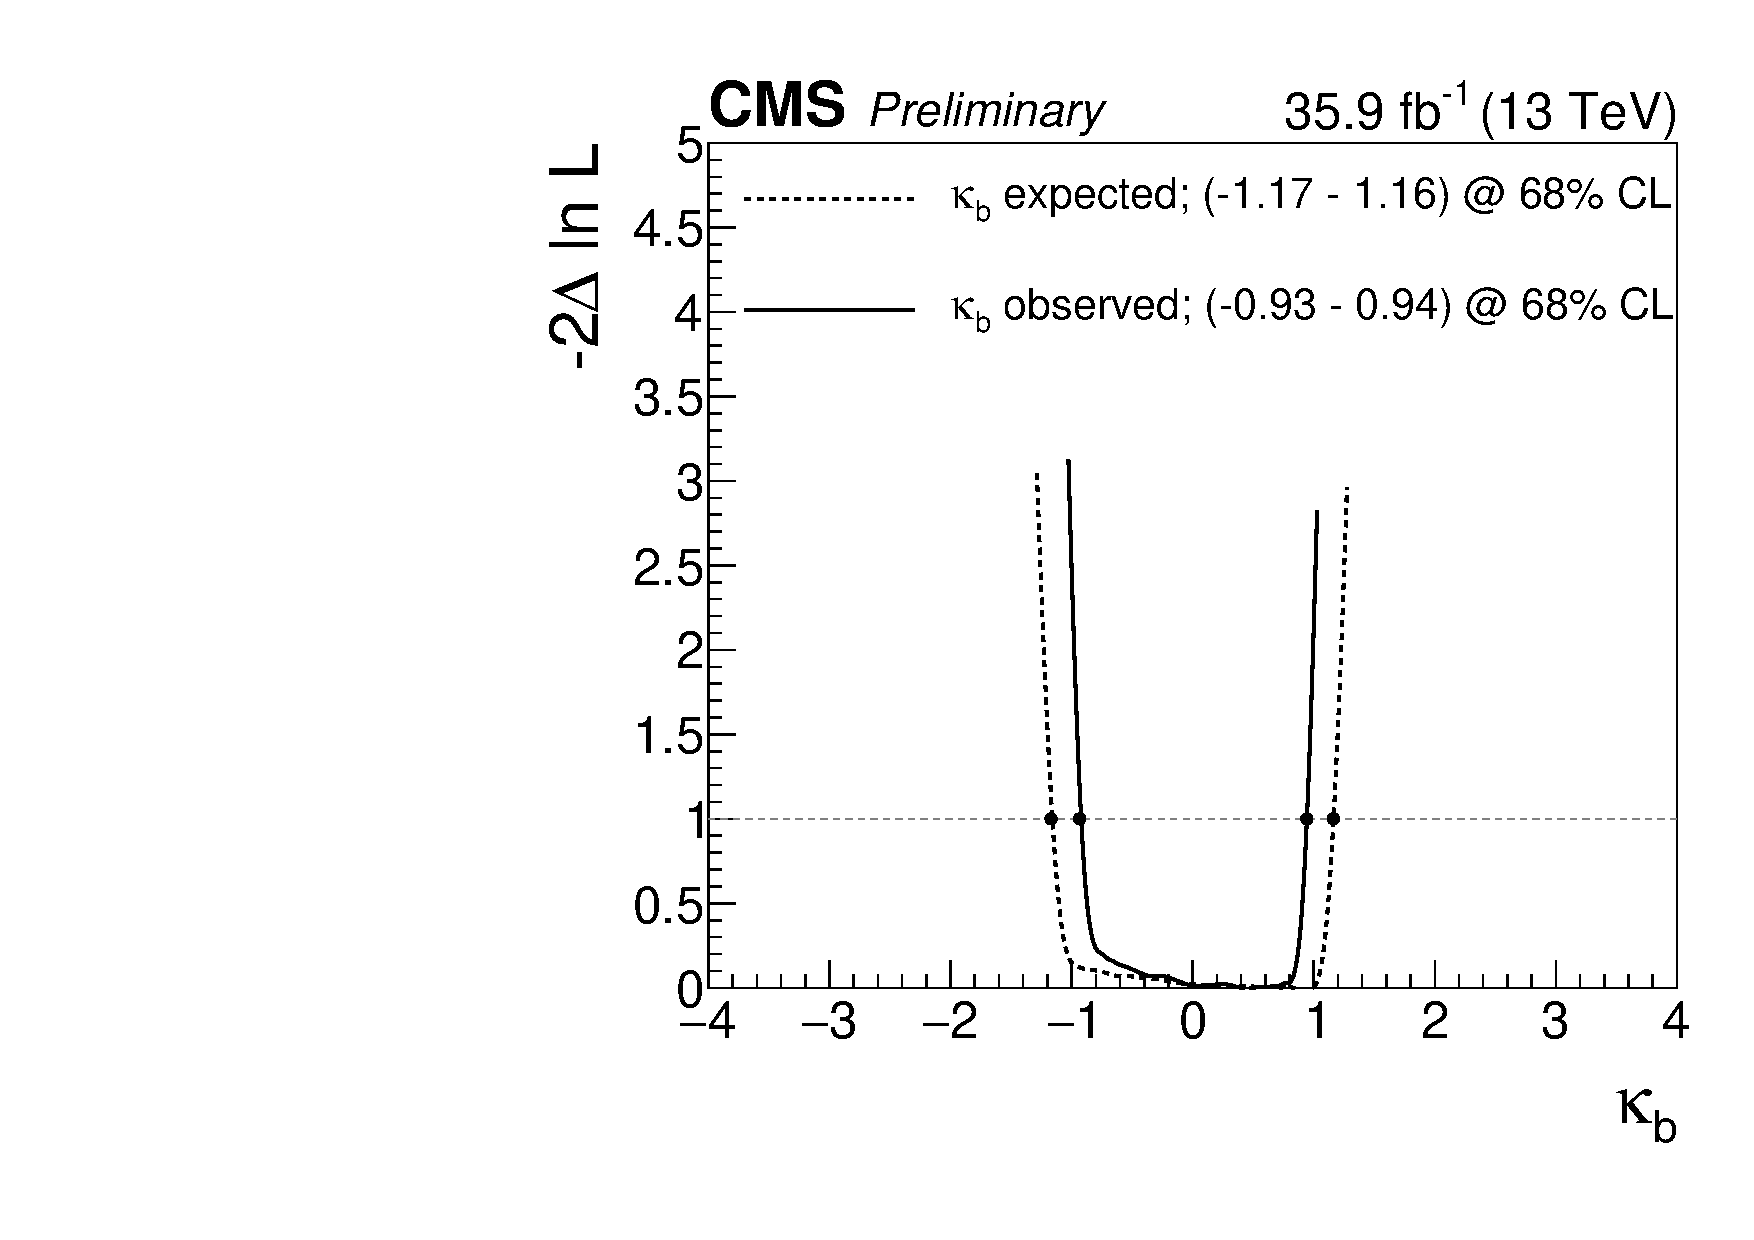
\includegraphics[width=\cmsFigWidth]{img/resultsapproval/reworked/onekappascan_kbkc_couplingdependentBRs_kappab.pdf}
    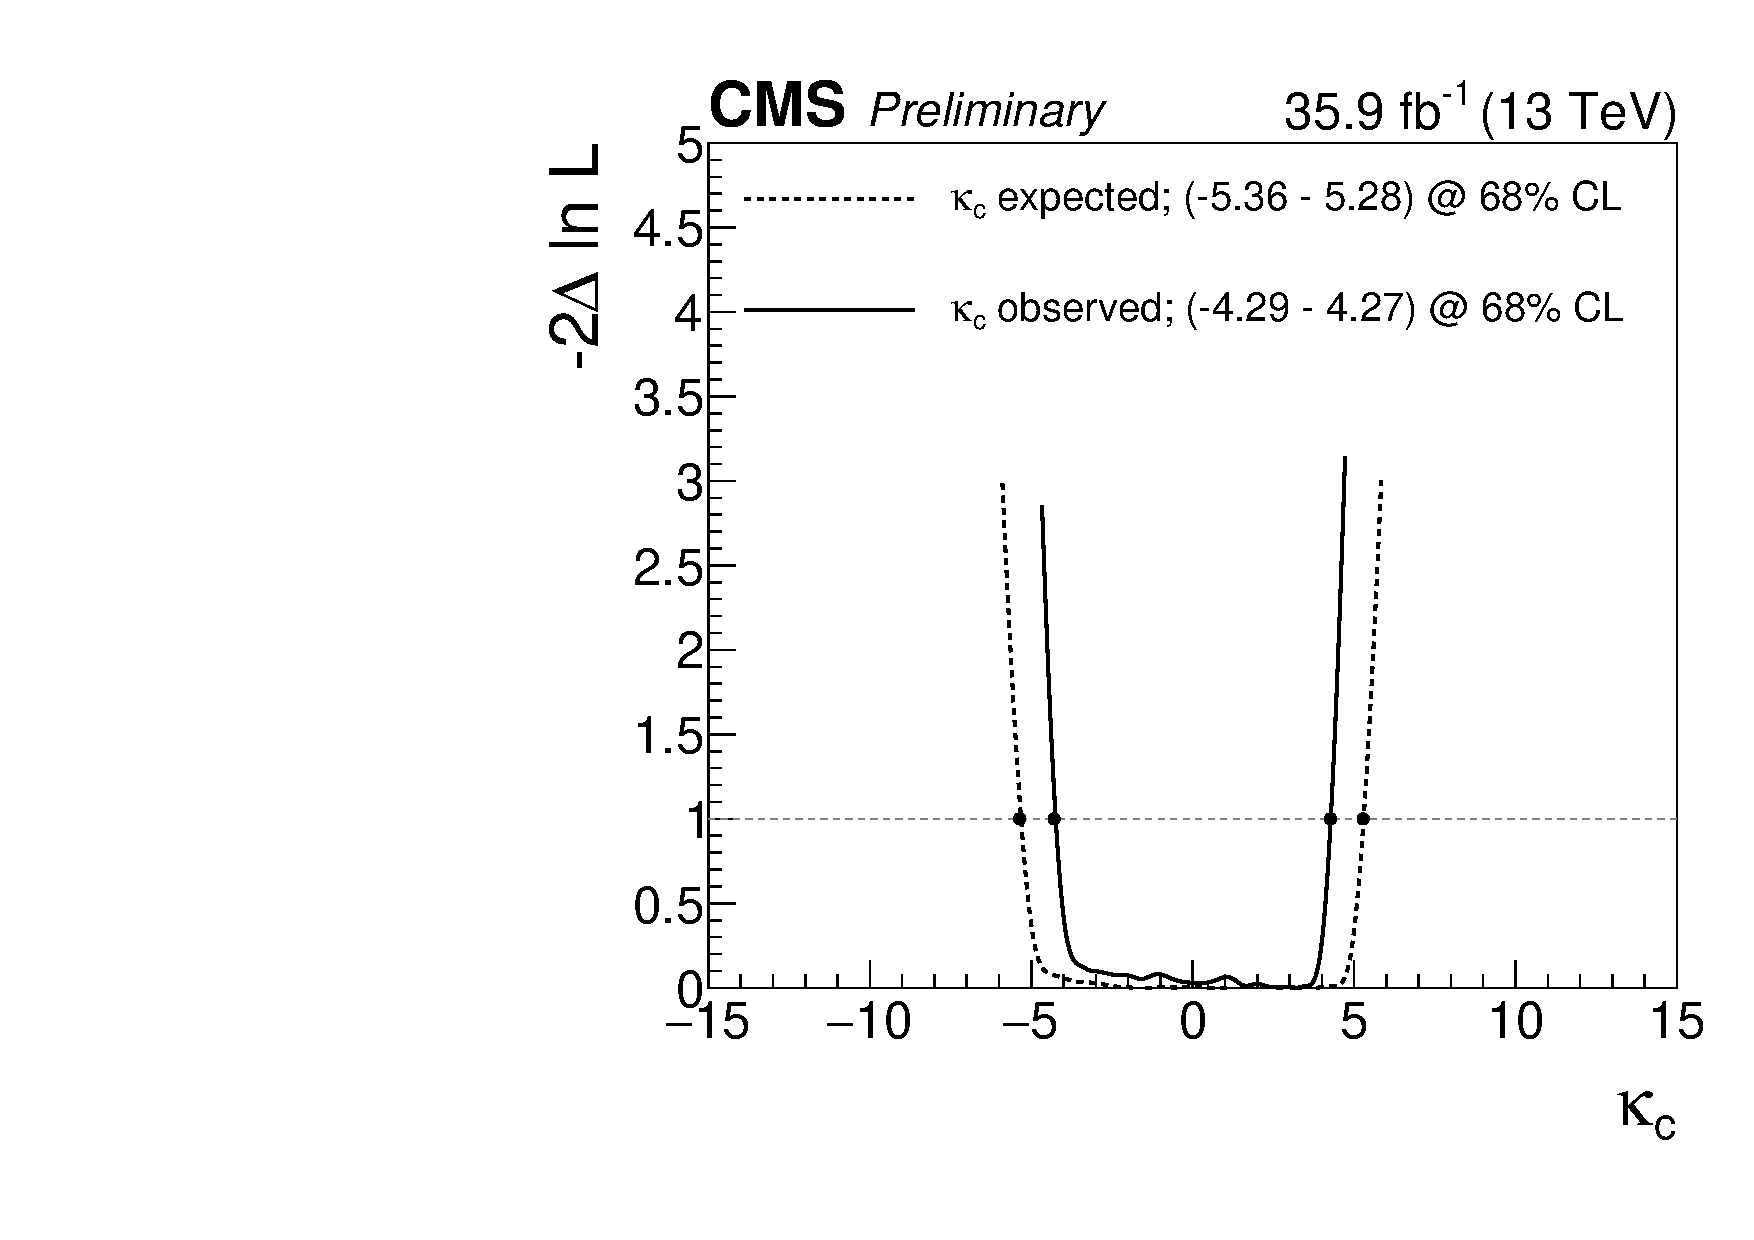
\includegraphics[width=\cmsFigWidth]{img/resultsapproval/reworked/onekappascan_kbkc_couplingdependentBRs_kappac.pdf}
    \caption{
        Scans of only one coupling, while profiling the other.
        % 
        The filled markers indicate the one standard deviation interval.
        % 
        The branching fractions were considered dependent on the values of the couplings.
        % 
        (\cmsLeft)
            Scan of $\kappa_b$ while profiling $\kappa_c$.
        (\cmsRight)
            Scan of $\kappa_c$ while profiling $\kappa_b$.
        }
    \label{fig:scans_kappabkappac_oneDimScans}
  \end{center}
\end{figure}

\begin{figure}[Hbtp]
  \begin{center}
    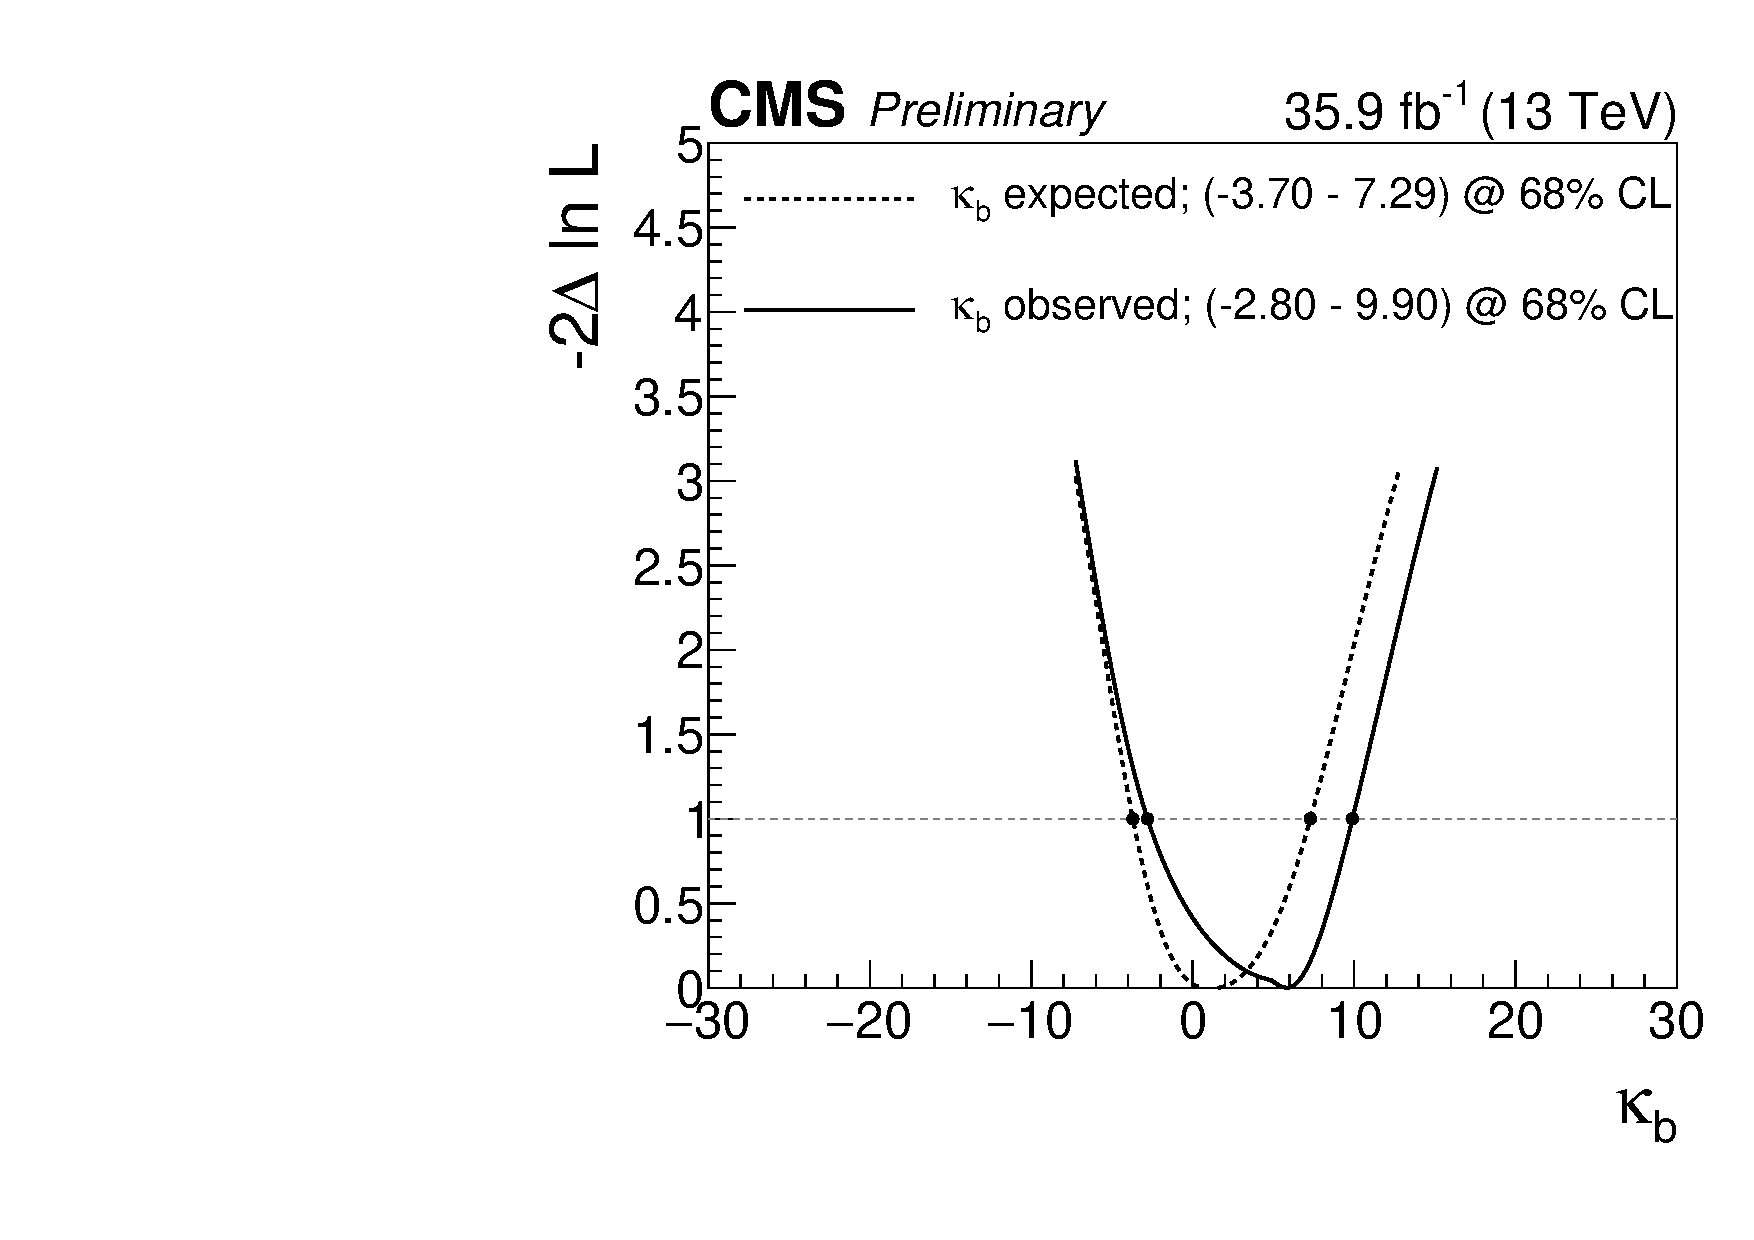
\includegraphics[width=\cmsFigWidth]{img/resultsapproval/reworked/onekappascan_kbkc_floatingBRs_kappab.pdf}
    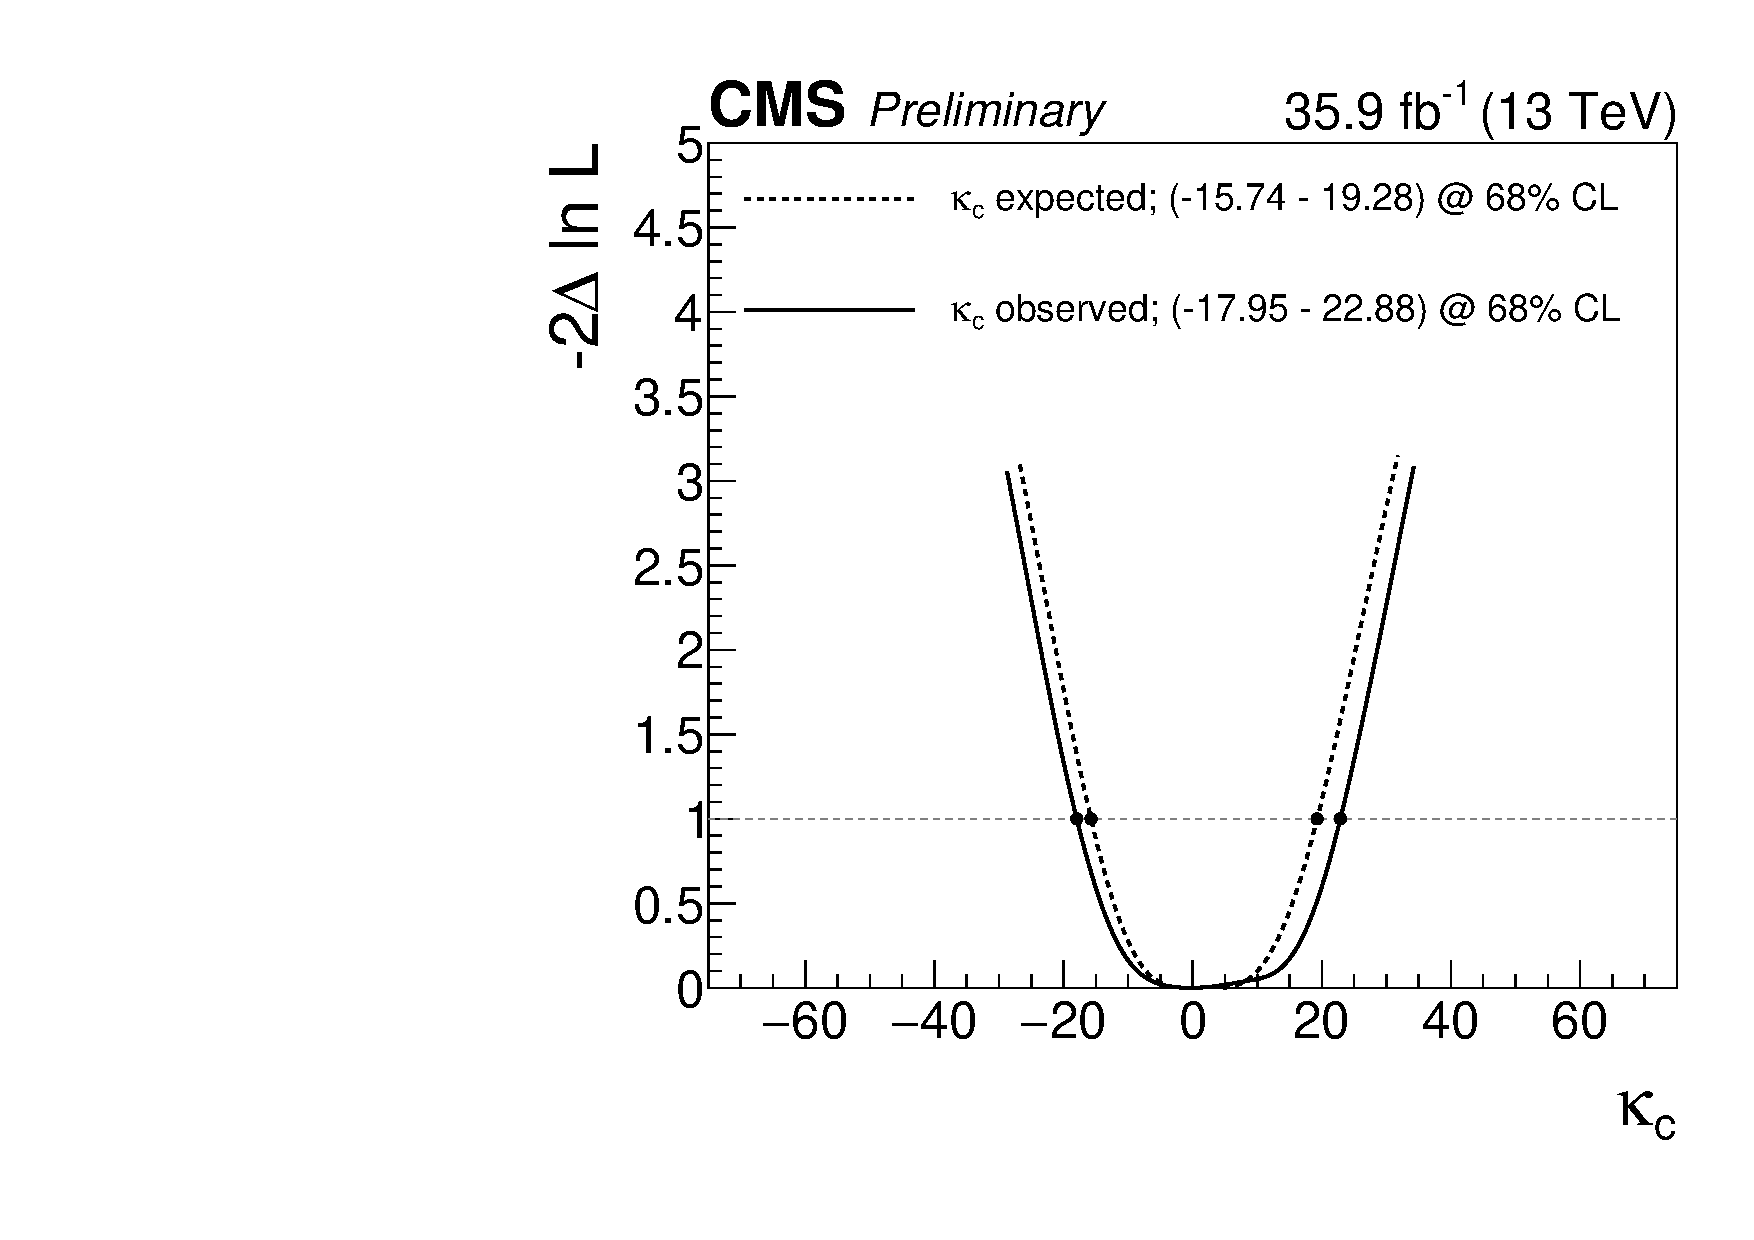
\includegraphics[width=\cmsFigWidth]{img/resultsapproval/reworked/onekappascan_kbkc_floatingBRs_kappac.pdf}
    \caption{
        Scans of only one coupling, while profiling the other.
        % 
        The filled markers indicate the one standard deviation interval.
        % 
        The branching fractions were freely floated in the fit.
        % 
        (\cmsLeft)
            Scan of $\kappa_b$ while profiling $\kappa_c$.
        (\cmsRight)
            Scan of $\kappa_c$ while profiling $\kappa_b$.
        }
    \label{fig:scans_kappabkappac_oneDimScans_scenario2}
  \end{center}
\end{figure}

% \clearpage
% \begin{equation}
%     s_i(\kappa_b, \kappa_c) =
%         \frac
%             {\sigma_i(\kappa_b, \kappa_c)}
%             {\sum_j \sigma_j(\kappa_b, \kappa_c)}
% \end{equation}







% ____________________________________________________________________________
\toggledclearpage
\subsection{Fits of Higgs coupling modifiers: \texorpdfstring{$\kappa_t$}{kt} vs. \texorpdfstring{$\cg$}{cg} and \texorpdfstring{$\kappa_t$}{kt} vs. \texorpdfstring{$\kappa_b$}{kb}}

% \begin{equation}
% \begin{align}
% % 
% s_i(\kappa_t, \cg)
%     &=
%     \frac
%         {\sigma_i(\kappa_t, \cg)}
%         {\sum_j \sigma_j(\kappa_t, \cg)}
%     \\
%     &=
%     \frac{
%         \sigma^\text{ggH}_i(\kappa_t, \cg) + \sigma^\text{xH}_i(\kappa_t, \cg)
%         }{
%         \sum_j \sigma^\text{ggH}_j(\kappa_t, \cg) + \sum_j \sigma^\text{xH}_j(\kappa_t, \cg)
%         }
%     \\
%     &=
%     \frac{
%         \sigma^\text{ggH}_i(\kappa_t, \cg) + \sigma^\text{xH}_i(\kappa_t, \cg)
%         }{
%         \sum_j \sigma^\text{ggH}_j(\kappa_t, \cg) + \sum_j \sigma^\text{xH}_j(\kappa_t, \cg)
%         }
%     %   
%     % 
%     % 
%     % \\
%     % &=
%     % \frac
%     %     {A_i \kappa_t^2 + B_i \cg^2 + C_i \kappa_t \cg}
%     %     {
%     %         \left(\sum_j A_j\right) \kappa_t^2
%     %         + \left(\sum_j B_j\right) \cg^2
%     %         + \left(\sum_j C_j\right) \kappa_t\cg
%     %         }
%     % \\
%     % &= 
%     % \frac
%     %     {A_i \frac{\kappa_t^2}{\cg^2} + B_i + C_i \frac{\kappa_t}{\cg}}
%     %     {
%     %         \left(\sum_j A_j\right) \frac{\kappa_t^2}{\cg^2}
%     %         + \left(\sum_j B_j\right) 
%     %         + \left(\sum_j C_j\right) \frac{\kappa_t}{\cg}
%     %         }
%     % \\
%     % &= f(\frac{\kappa_t}{\cg})
% % 
% \end{align}
% \end{equation}


The fits are repeated in a way analogous to that of Sec.~\ref{sec:ResultsKappabKappac} but with $\kappa_t$, $\cg$ and $\kappa_b$ as the parameters of the fit, using the parametrization obtained from Ref.~\cite{Grazzini:2017szg}.
% 
% Analogous to Sec.~\ref{sec:ResultsKappabKappac}, the fits are repeated with now $\kappa_t$, $\cg$ and $\kappa_b$ and as the fitted parameters, using the parametrization obtained from Ref.~\cite{Grazzini:2017szg}.
% 
The combined log-likelihood scan for $\kappa_t$ vs. $\cg$, assuming branching fractions that depend on the couplings, is shown in Fig.~\ref{fig:scans_kappatkappag_nominal}(\cmsLeft).
% 
The normalization of the spectrum is, by construction, equal to the SM normalization for the points $( \kappa_t = 1.0, \cg = 0.0 )$ and $( \kappa_t = 0.0, \cg \simeq 0.08 )$.
% 
The differential shape of the parametrization $s$ is calculated by normalizing the differential cross section to one:
% 
% \clearpage
\begin{equation}
    s_i(\kappa_t, \cg) =
        \frac
            {\sigma_i(\kappa_t, \cg)}
            {\sum_j \sigma_j(\kappa_t, \cg)}
    \,,
\end{equation}
% 
where $\sigma_i$ is the parametrization in bin $i$.
% 
Further simplification %
% 
% \footnote{
%     $
%     s_i(\kappa_t, \cg)
%         =
%         \frac
%             {\sigma_i(\kappa_t, \cg)}
%             {\sum_j \sigma_j(\kappa_t, \cg)}
%         =
%         \frac
%             {A_i \kappa_t^2 + B_i \cg^2 + C_i \kappa_t \cg}
%             {
%                 \left(\sum_j A_j\right) \kappa_t^2
%                 + \left(\sum_j B_j\right) \cg^2
%                 + \left(\sum_j C_j\right) \kappa_t\cg
%                 }
%         = 
%         \frac
%             {A_i \frac{\kappa_t^2}{\cg^2} + B_i + C_i \frac{\kappa_t}{\cg}}
%             {
%                 \left(\sum_j A_j\right) \frac{\kappa_t^2}{\cg^2}
%                 + \left(\sum_j B_j\right) 
%                 + \left(\sum_j C_j\right) \frac{\kappa_t}{\cg}
%                 }
%         = f(\frac{\kappa_t}{\cg})
%     $
%     }
% 
reveals that the shape of the parametrization for $\kappa_t$/$\cg$ variations becomes a function of the ratio of the two couplings, $s_i(\frac{\kappa_t}{\cg})$.
% 
Thus any discrimination power in the radial direction with respect to the origin stems from constraints on the overall normalization, whereas discrimination in the angular direction stems from constraints on the shape of the distribution.
% 
The angular dependence of the log-likelihood function becomes apparent in Fig.~\ref{fig:scans_kappatkappag_nominal}(\cmsRight), where the branching fractions were freely floated in the fit.
% 
Except at small values of the couplings, the constraint on the couplings depends on their ratio.
% 
The two symmetric sets of contours are due to a symmetry of the parametrization under $(\kappa_t,\,\cg) \, \to \, (-\kappa_t,\,-\cg)$.


\begin{figure}[hbtp]
  \begin{center}
    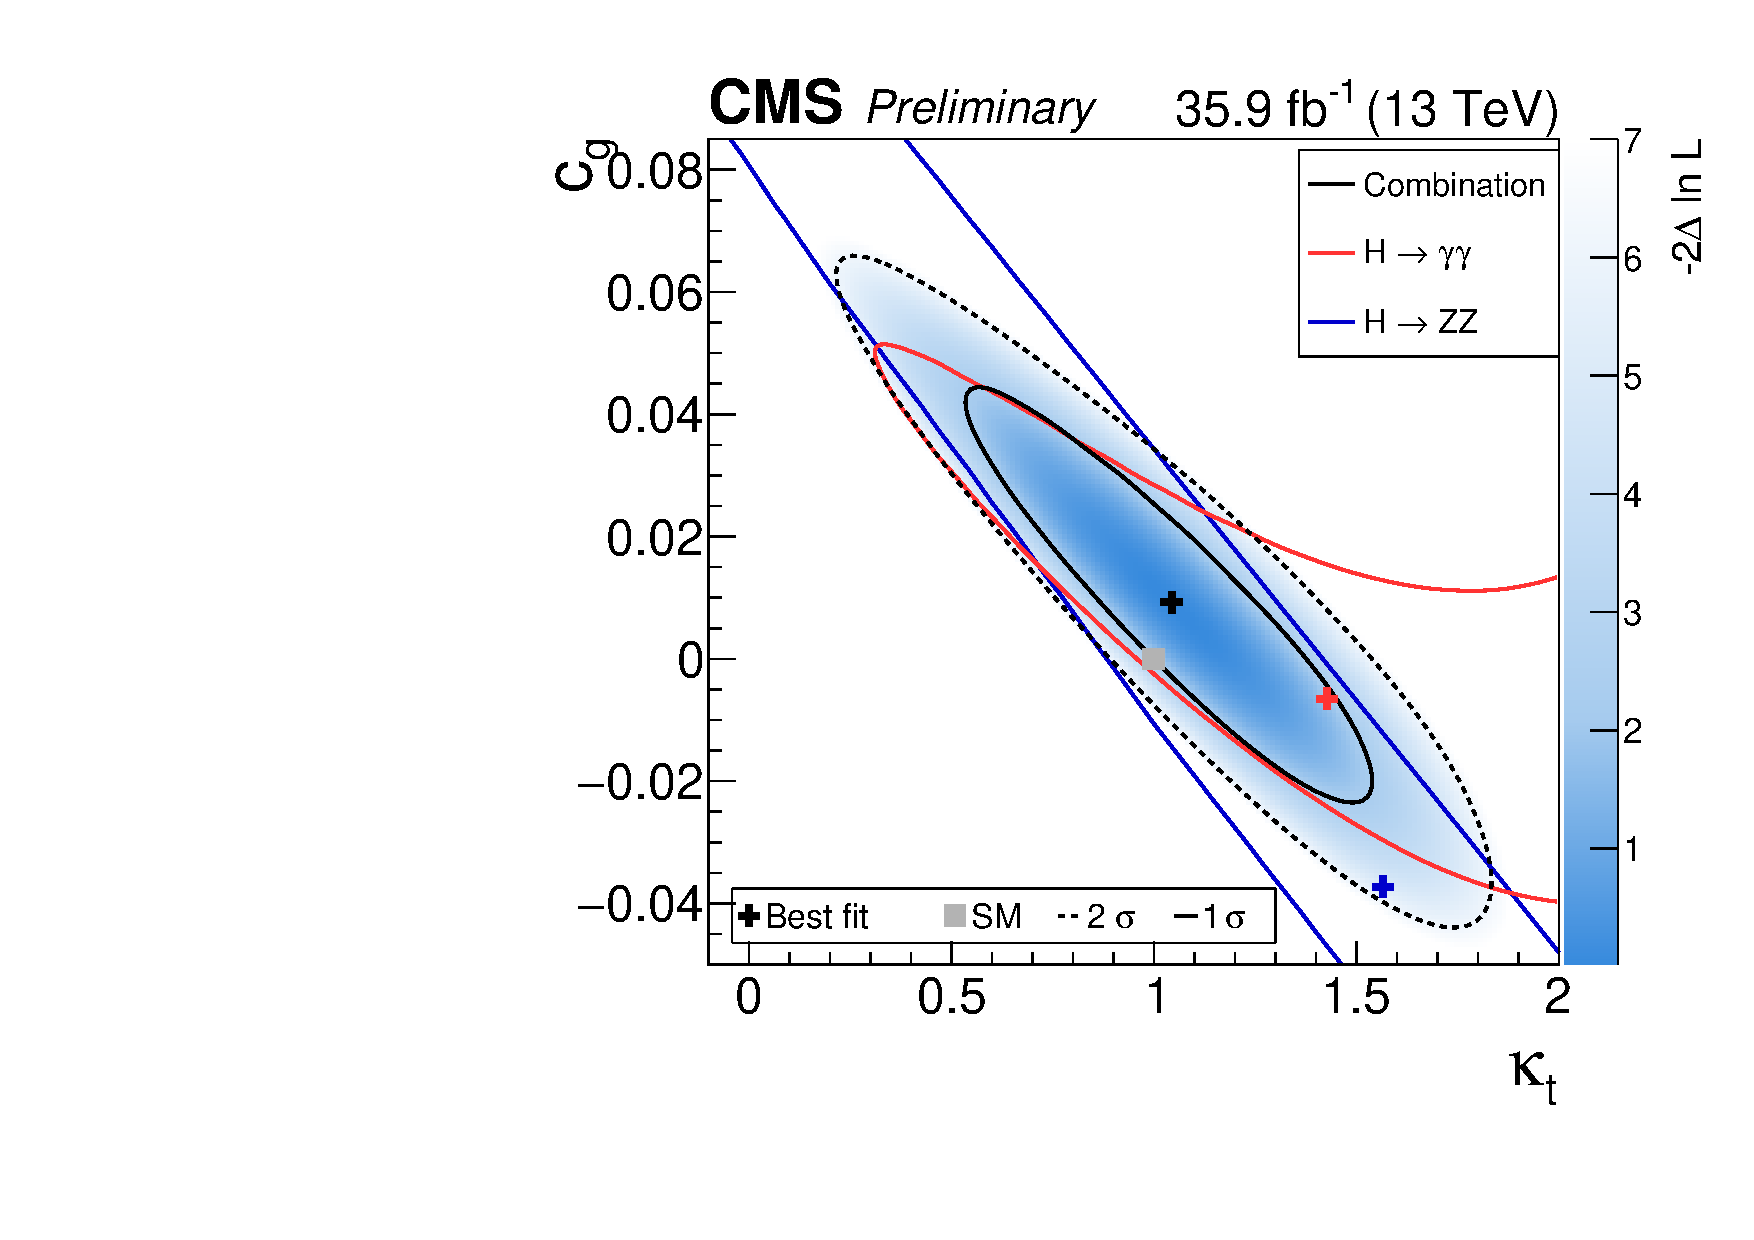
\includegraphics[width=0.49\linewidth]{img/resultsapproval/reworked/multicont_ktcg_couplingdependentBRs.pdf}
    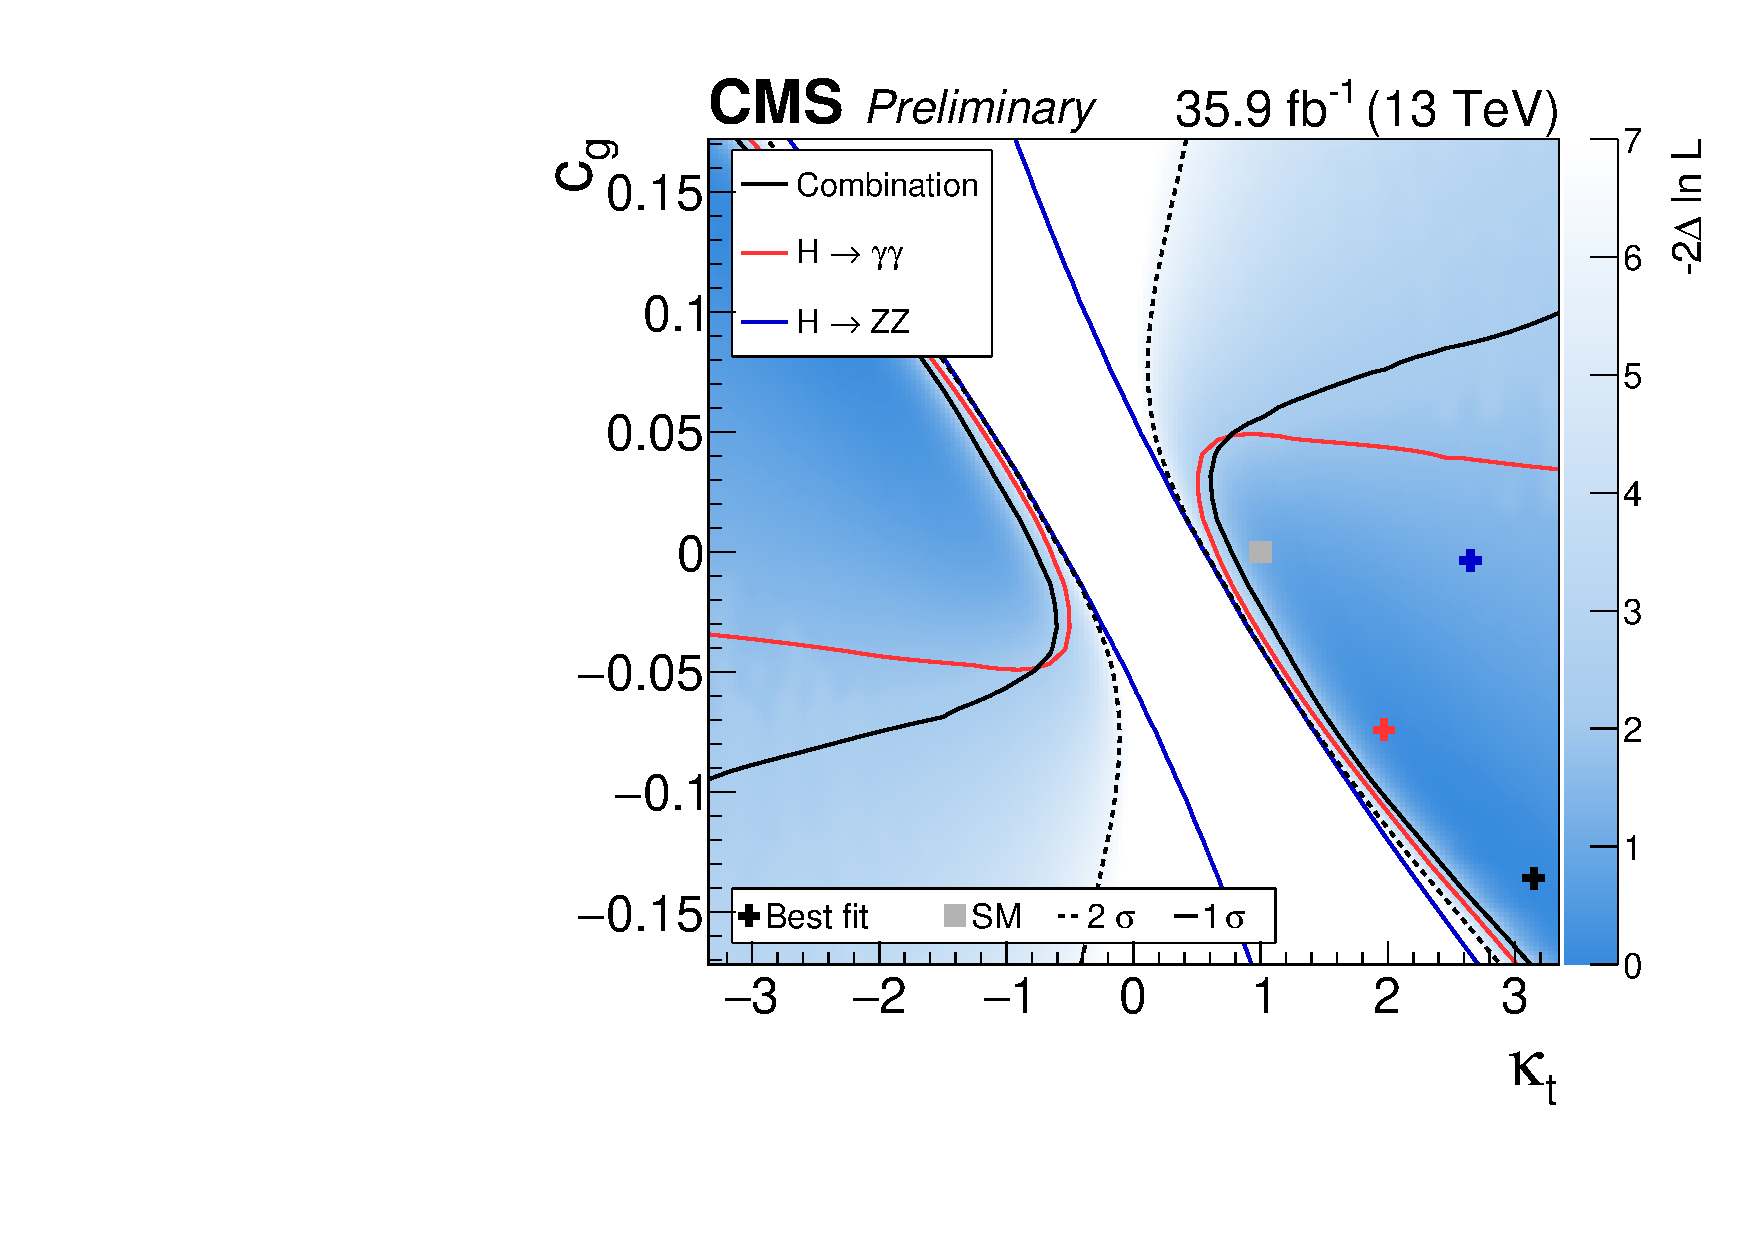
\includegraphics[width=0.49\linewidth]{img/resultsapproval/reworked/multicont_ktcg_floatingBRs.pdf}
    % 
    \caption{
        Simultaneous fit results for $\kappa_t$ and $\cg$.
        % 
        (\cmsLeft)
        % 
        One and two standard deviation contours are shown for the combined ($\hgg$, $\hzz$ and $\hbb$) fit to data and for $\hgg$ and $\hzz$ separately, assuming a coupling dependency of the branching fractions.
        % 
        % \arc{Fig.8 You don’t include Hbb alone because the uncertainty is too big ? How much is it ?}
        % \tk{Include $\hbb$-only}
        % 
        % (\cmsRight) The log-likelihood as a function of the angle in the $\kappa_t$-$\cg$ plane, letting the branching fractions float freely in the fit.
        % 
        (\cmsRight) One and two standard deviation contours are shown for the combined ($\hgg$, $\hzz$ and $\hbb$) fit to data and for $\hgg$ and $\hzz$ separately, assuming freely floating branching fractions.
        }
    \label{fig:scans_kappatkappag_nominal}
  \end{center}
\end{figure}


Figure~\ref{fig:scans_kappatkappab_rawInput}(\cmsLeft) shows the combined log-likelihood scan as a function of $\kappa_t$ and $\kappa_b$, with branching fractions scaling appropriately with the coupling modifiers and Figure~\ref{fig:scans_kappatkappab_rawInput}(\cmsRight) with freely floating branching fractions.
% 
As the $\hgg$ branching fraction depends linearly on $\kappa_t$, the constraints on $\hgg$ and the combination in Figure~\ref{fig:scans_kappatkappab_rawInput}(\cmsLeft) are not symmetric with respect to the $\kappa_t$-axis.
% 
For freely floating branching fractions, the parametrization is symmetric under $(\kappa_t,\,\kappa_b) \, \to \, (-\kappa_t,\,-\kappa_b)$, which explains the observed symmetry in in Figure~\ref{fig:scans_kappatkappab_rawInput}(\cmsRight).

\begin{figure}[hbtp]
  \begin{center}
    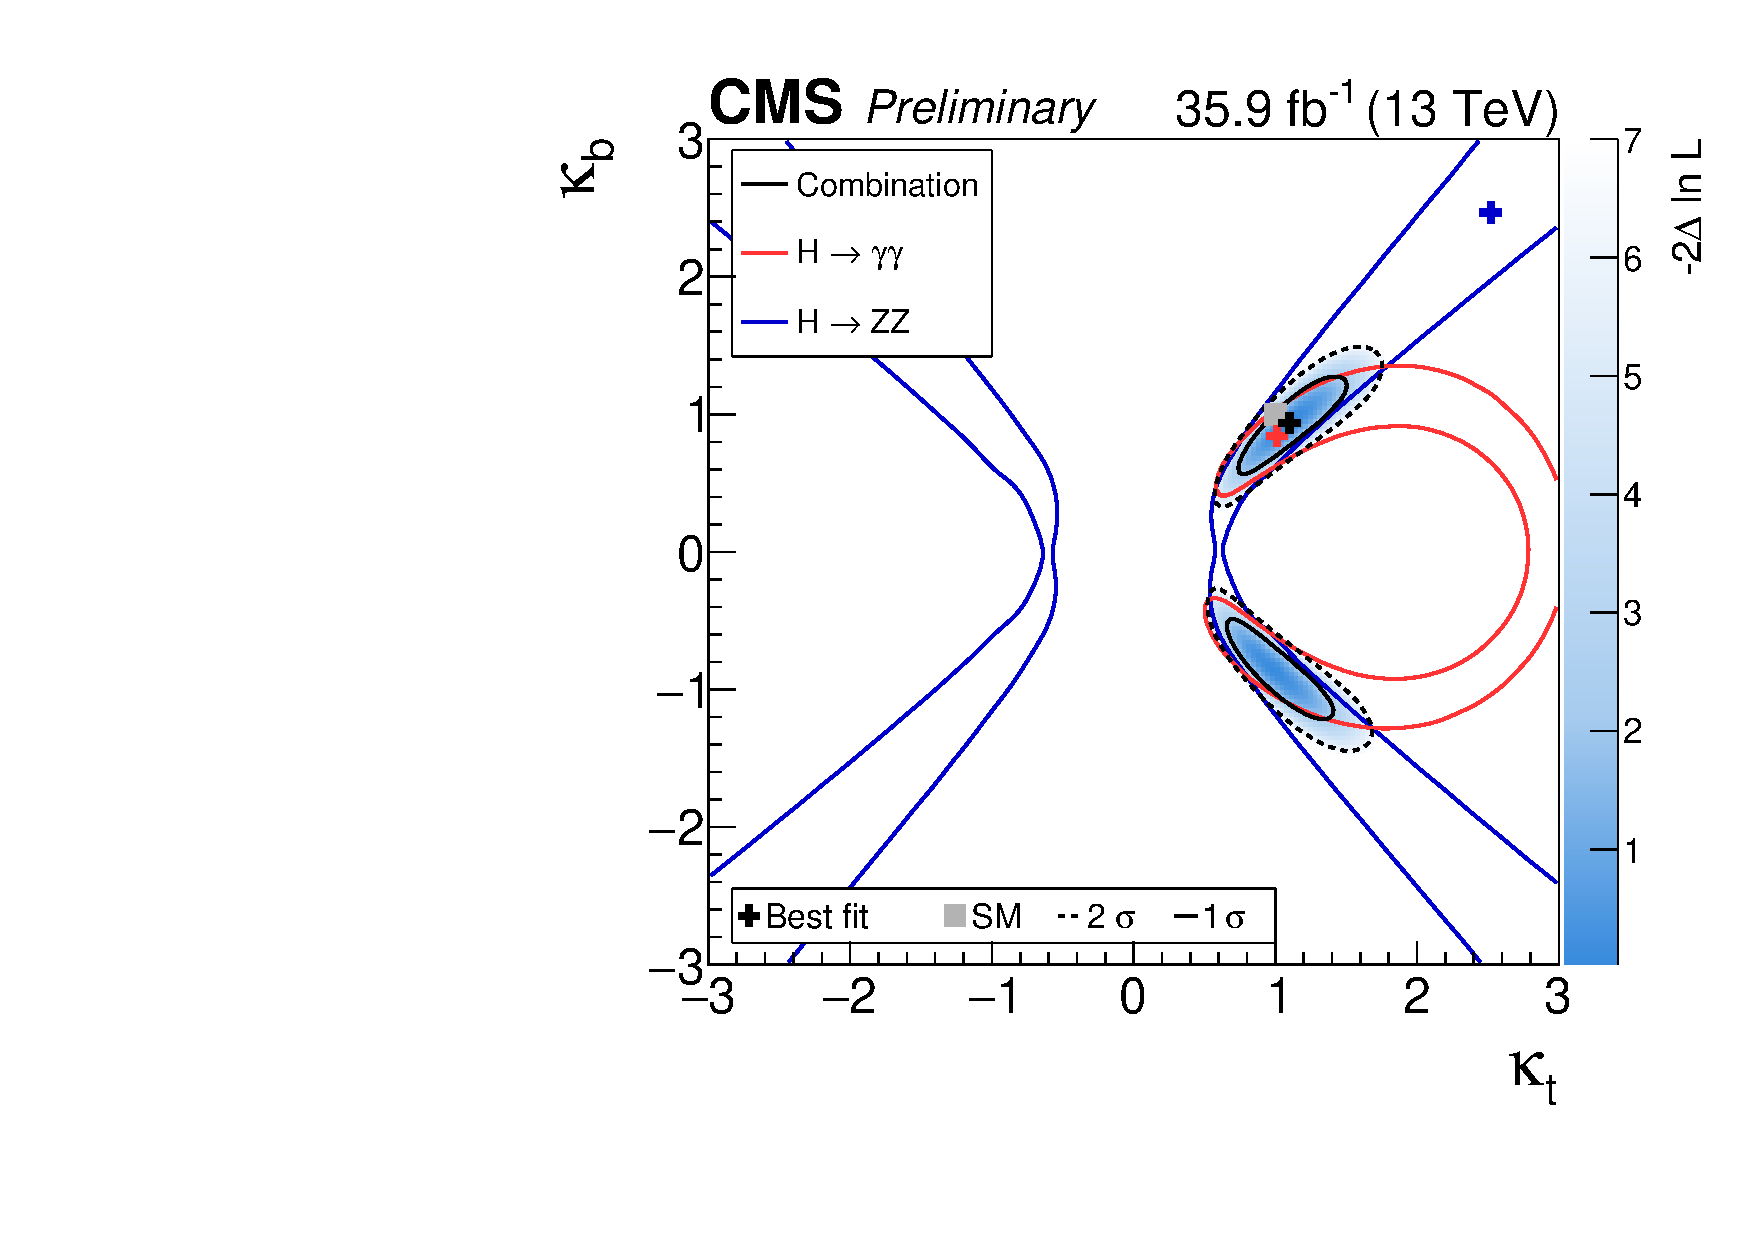
\includegraphics[width=0.49\linewidth]{img/resultsapproval/reworked/multicont_ktkb_couplingdependentBRs.pdf}
    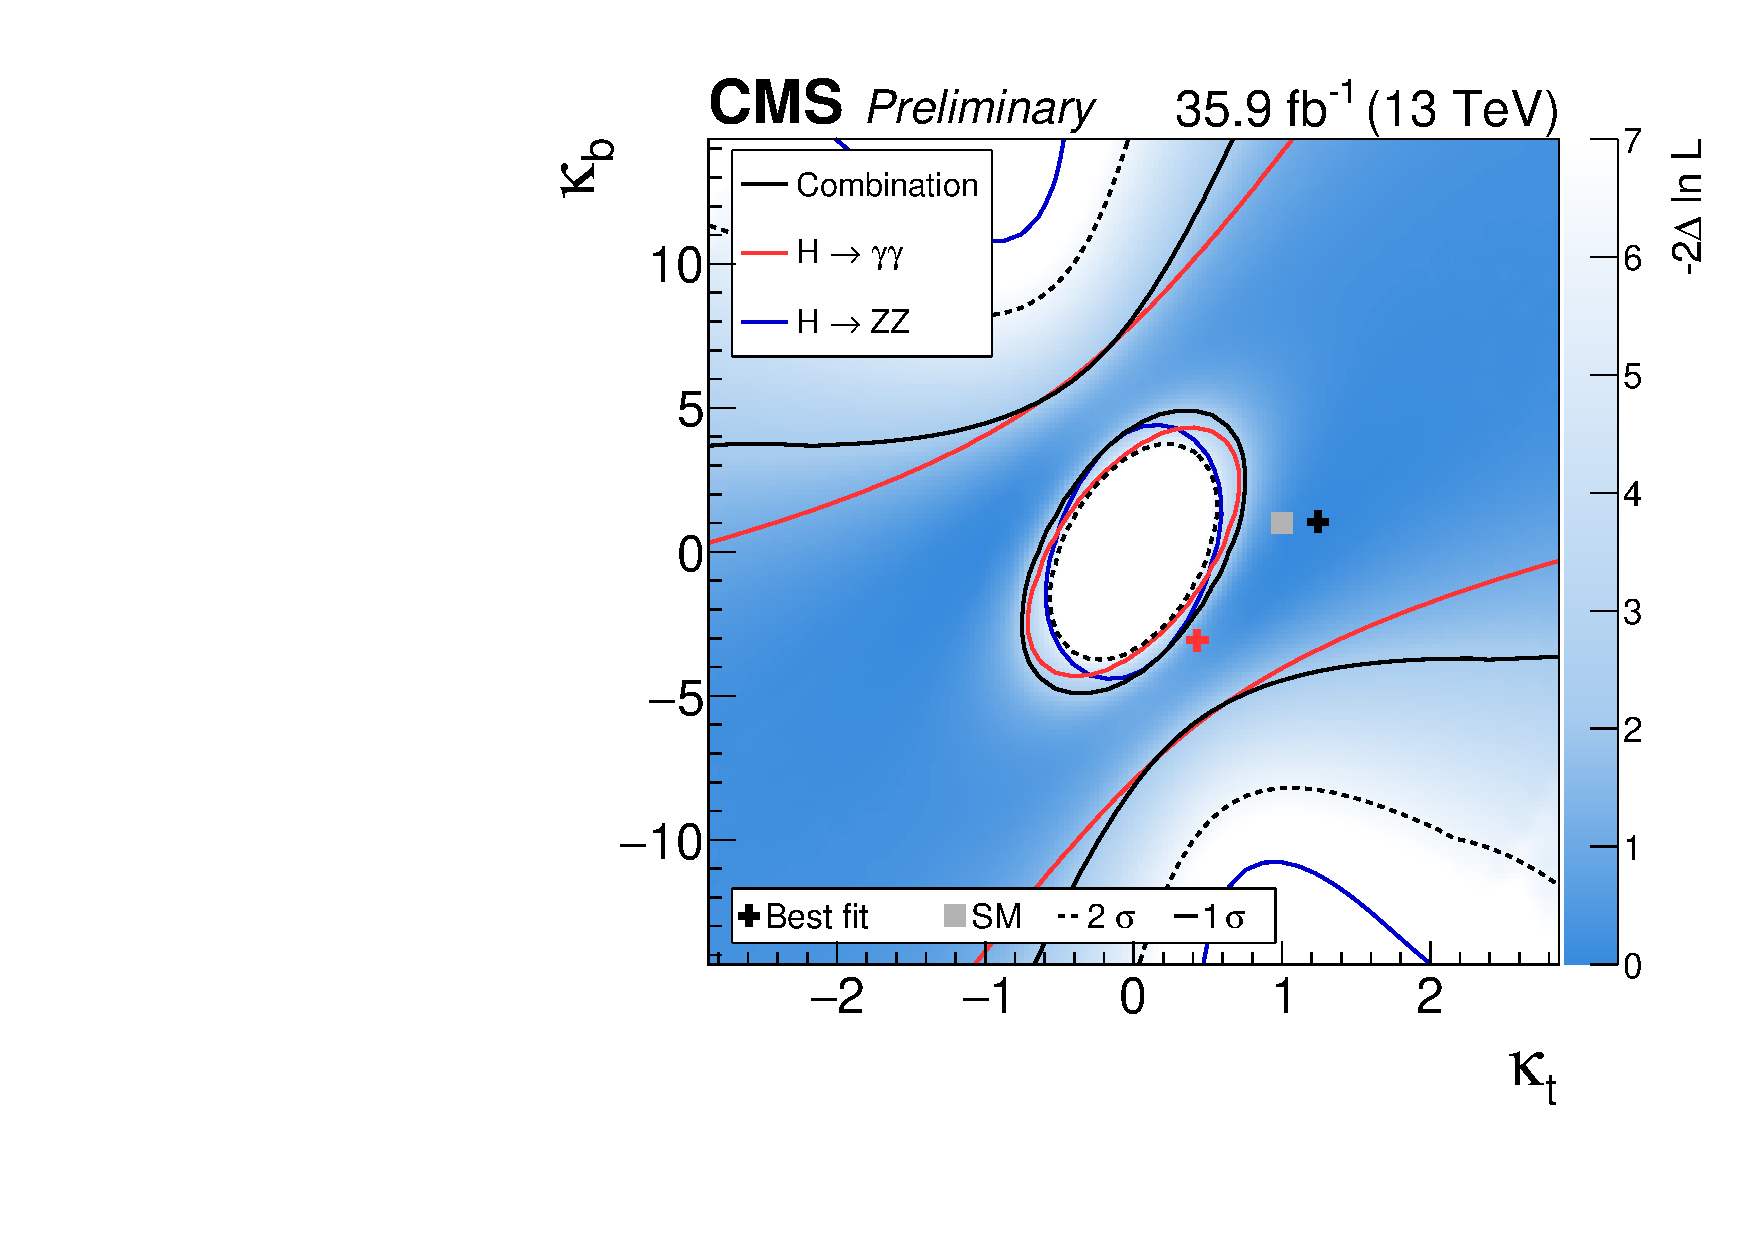
\includegraphics[width=0.49\linewidth]{img/resultsapproval/reworked/multicont_ktkb_floatingBRs.pdf}
    % 
    \caption{
        Simultaneous combined fit results for $\kappa_t$ and $\kappa_b$.
        % 
        (\cmsLeft) One and two standard deviation contours are shown for the combined ($\hgg$, $\hzz$ and $\hbb$) fit to data and for $\hgg$ and $\hzz$ separately, assuming a coupling dependency of the branching fractions.
        % 
        (\cmsRight) One and two standard deviation contours are shown for the combined ($\hgg$, $\hzz$ and $\hbb$) fit to data and for $\hgg$ and $\hzz$ separately, where the branching fractions were freely floated in the fit.
        }
    \label{fig:scans_kappatkappab_rawInput}
  \end{center}
\end{figure}



